%!TEX root = ../../main.tex
\renewcommand{\appendixname}{Appendix~}
\appendix
\section{アリフィフティ}
日本人は古来より礼節を重んじてきた。
海外に比べ「すいません」を多用する民族として知られており、なぜ日本人はここまで謝るのかと疑問を持たれていることであろう。
この「すいません」は外国語に逐語訳することは不可能であり、たとえば店員を呼ぶときの「すいません」は「Excuse me./Sir」であり、「すいません、お手数おかけします」は「Thank you very much」で十分である。
このように、日本語は他人に対して、端から見れば不必要なほど敬意を払う言語であるが、それが日本語の美学である。
その多様性を裏付けるかのように、表現方法が様々にあるのが事実である。
特に礼節に関する「ありがとう」は殊更多くの表現がある。
\begin{itemize}
\item 御礼申し上げます
\item ありがとうございます
\item ありがとう
\item あざっす
\item あざ
\end{itemize}
ここに挙げた以外にも表現方法は考えられると思うが、代表的なものを挙げた。
また、礼を述べる際の一種の照れを隠すために、いわゆるオヤジギャク(駄洒落)を交えて述べることも見受けられる。
\begin{itemize}
\item 蟻が10匹、蟻が10(ありがとう)
\end{itemize}
ここには相手に対して、働き者として知られている蟻を10匹集めて、今後あなたにお使えします、との意味も込められていると考えられており、一般的な「ありがとう」よりもより高度な礼節に関する表現であると論じる学説もあるほどである。
このように、一般的に蟻が10匹集まると、他人に対して英語で「$thank\ you\ very^{10}\ much$」の意を表す(10はveryに対する指数)、日本語として最上級の挨拶を表すことができる。

\par

近年、このveryの指数をより高次元に拡張できないかを論じる現代数学の最先端の学説である「アリフィフティ学」が頻繁に議論されている。
アリフィフティ学を理解・議論するためには、非常に高度な数学の知識が必要であり、その詳細はアリフィフティ学を論ずる論文に譲ることとする。
誤解を恐れずにその概念を説明するのであれば、蟻次元空間に蟻を複数匹$(10<n<50)$集めた場合に、どのような基底状態が考えられるかを研究する学問である。
これまでの挨拶は$n=10$の場合(これは特別蟻解と呼ばれる)である。
蟻の上限値は49匹に設定されており、50匹集まった場合には、現代数学の解釈上はアリフィフティ・エフェクトと呼ばれ、アリフィフティ第二公式の積分値が発散することが知られており、蟻は集めてもいいが49匹までに留めることが現実的な議論であるとされている。
しかし、50匹を集めるべきであるという蟻学者の主張もあいまって、$n=50$を実現するためにどうすればいいかを議論するのがアリフィフティ学の目的の一つである。
アリフィフティ第一公式は、
\[
F = A \times n\  (10<n<50)
\]
である。ここで、$F$はfifytyの頭文字であり、集められた蟻の個体値を表す。
$A$は蟻仕事関数と呼ばれ、集めることのできた蟻の働き具合に関連する量であり、一般的に働き蟻のやる来に相当する。
$n$は実際に集められた蟻の個体数に相当する(4次元空間の挨拶に変換する際は、蟻次元空間の量である$n$を蟻次元変換ファクターと呼ばれる変換公式を用いる必要がある)。
この議論からも分かるように、例えば$A \simeq 100 $の非常に高度な技術を有する蟻(いわゆる「百人力(正確には百蟻力)」)を1匹だけ集めた場合、
\[
F = 100 \times 1 = 100
\]
となる。
第一公式の計算自体は、非常に単純であるが、蟻の働き具合を表す$A$をいかにして精度良く求めるかが重要である。
このアリフィフティ学は未完成であり、完成した際には、その解を4次元空間の量へと変換すれば日本語の特性を示すことになり、また蟻次元空間で解釈すれば、いかに蟻が働き者かを論ずることができ、「アリとキリギリス」のグリム童話の裏付けをとることができる。

\par

このように高度な学問であるため、しばしアリフィフティ学者のやり取りに、一人無知をさらすサラリーマンが紛れ込んでいるのも事実である。
図\ref{fig:Ari50}に、アリフィフティ学会におけるやり取りを示す。
希望新風とは、アリフィフティ学会に新風を吹き荒らすごとく登場した期待の新人学者であるが、又吉・竹田の古くから研究している両者の会話のレベルにはついてこれなかった様である。

\begin{figure}[htbp]
 \begin{minipage}{0.5\hsize}
  \begin{center}
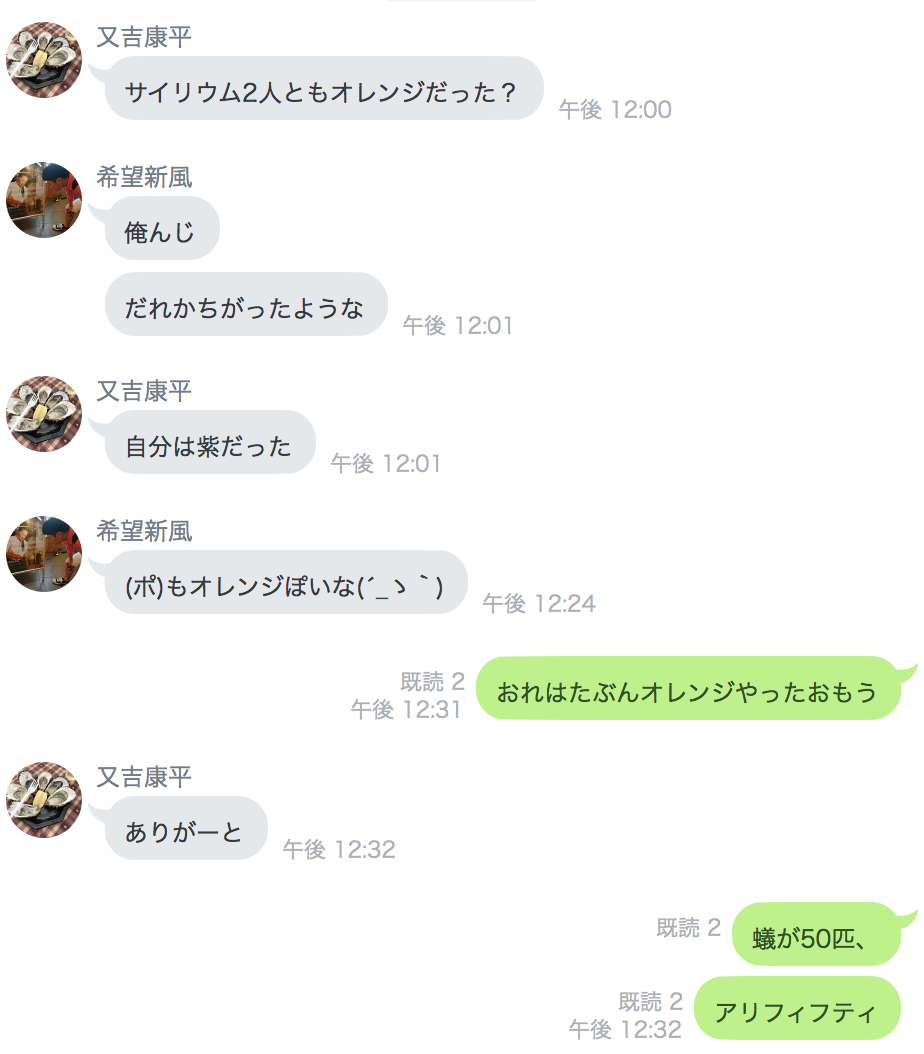
\includegraphics[width=0.8\textwidth]{./section/Appendix/figures/ari50_1.png}
  \end{center}
  \label{fig:one}
 \end{minipage}
 \begin{minipage}{0.5\hsize}
  \begin{center}
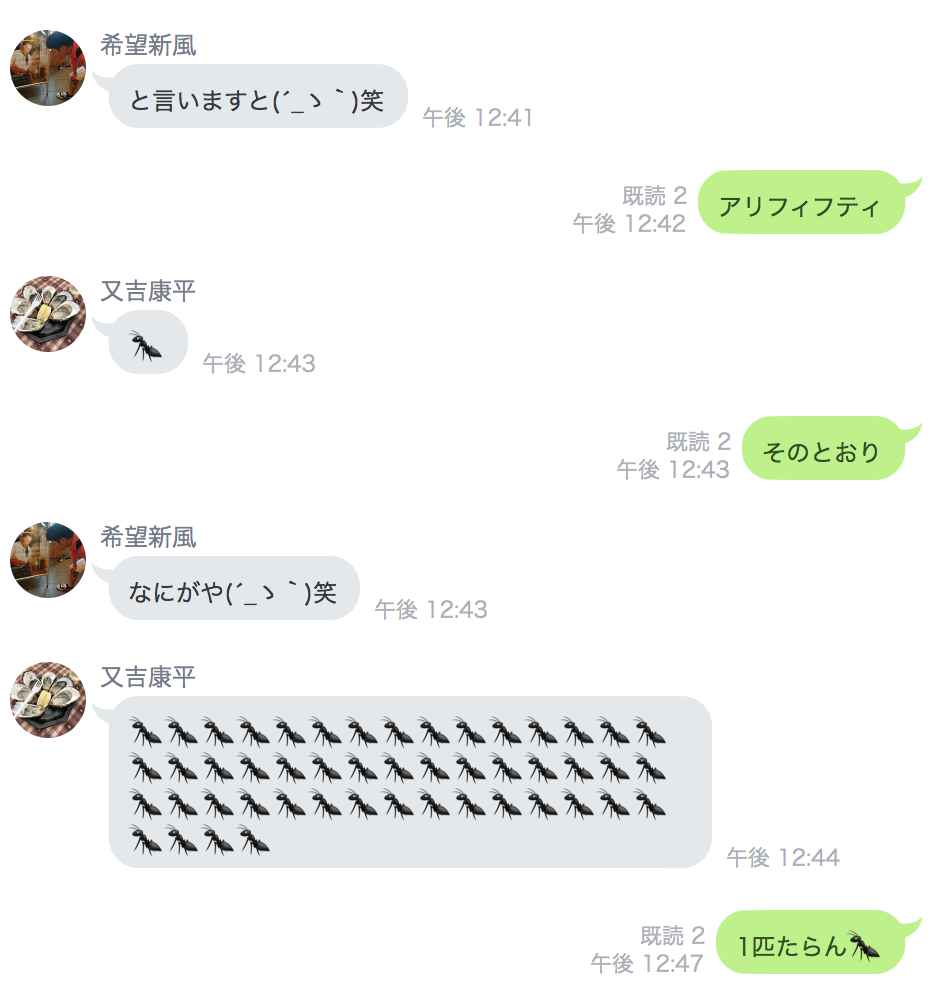
\includegraphics[width=0.8\textwidth]{./section/Appendix/figures/ari50_2.png}
  \end{center}
 \end{minipage}
 \caption{アリフィフティ研究学にまざる素人}
  \label{fig:Ari50}
\end{figure}

以上の議論を踏まえると、
\[
蟻が50匹、
アリフィフティ
\]
に対して又吉清掃員は蟻の1匹だけの絵文字を送ってきた。
これは、$n=49$で現状とどまっているアリフィフティ学に足りないのは、あと1匹であるということを示しており、
最後の竹田研究員の「1匹足らん」は、我々はアリフィフティ学を研究しているため、$n=50$を主張すべきだと批判しているのである。
最後に、サラリーマンに対するツッコミへの批評をしてこの章を締めくくることにする。
そう、「と言いますと」ではなく、「50匹集まったら積分が発散するでしょうが」とツッコむのが正解であったのだ。ここまで読んでくれて、アリフィフティ。
\par
いま心の中で「発散しとるやないか」と突っ込めたあなたは立派な蟻学者になれるであろう。




%~~~~~~~~~~~~~~~~~~~~~~~~~~~~~~~~~~~~~~~~~~~~~~~~~~
\newpage
\section{ガスヒーポン}


\newpage 
\section{ワールドカップ}
%=====================%
\section{スポーツ観戦}
%=====================%
これまで数々の非言語の概念を研究してきたが、非言語と現実の事象との関係性は研究されてこなかった。
ここでは新しい研究手法を取り入れ、非言語と現実言語の比較に成功した。

\begin{table}[htb]
  \centering
  \caption{2018年6月19日(火)ワールドカップ初戦}
  \label{my-label}
  \scalebox{0.5}[0.5]{
    \begin{tabular}{|l|l|l|l|l|l|} \hline
      試合経過  & コロンビア                                   & 日本                                 & 草原理論  \\ \hline \hline
                &                                              &                                       & サッカーはじまる\sf(´\_ゝ`)笑 \\ \hline \hline
      前半03分  &                                              & 大迫の左足シュートはゴールを阻まれる  &                                  \\ \hline
      前半03分  &                                              & 香川の左足シュートは枠外              &                                  \\ \hline
      前半03分  & C・サンチェスが得点機会阻止(手)により即退場 &                                       &                                   \\ \hline
      前半06分  &                                              & ゴール!! 香川の1号                 & きた!!!!おおおぉぉにゅお  \\ \hline
                &                                              &                                       & なんやこの展開おもんない\sf (´\_ゝ`)笑\\ \hline
                &                                              &                                       & これは勝つ\sf (´\_ゝ`)笑\\ \hline
      前半12分  & ファルカオの右足シュートはゴールを阻まれる   &                                       &   \\ \hline
      前半15分  &                                              & 乾の右足シュートは枠外                &    \\ \hline
      前半16分  & キンテロの左足シュートは枠外                 &                                       & \\ \hline
      前半26分  & Ju・クアドラードの右足シュートは枠外       &                                       & \\ \hline
      前半31分  & Ju・クアドラードがアウト、バリオスがイン   &                                       & \\ \hline
      前半32分  &                                              & 大迫の右足シュートは枠外              & \\ \hline
      前半34分  & ファルカオの右足シュートはゴールを阻まれる   &                                       & \\ \hline
      前半39分  & ゴール!! キンテロの1号                    &                                       & なんやこれ\sf (´\_ゝ`)笑\\ \hline
                &                                              &                                       & ださい\sf (´\_ゝ`)笑\\ \hline
                &                                              &                                       & あのフリーキックのファールはおかしいんではっっ\sf (´\_ゝ`)笑\\ \hline
                &                                              &                                       & やとしてもなぜ川島は真横に飛ばなかったのか\sf (´\_ゝ`)笑笑 \\ \hline
                &                                              &                                       & オォォヌゥ\sf (´\_ゝ`)笑 \\ \hline
                &                                              &                                       & ばららららららら\sf (´\_ゝ`)笑 \\ \hline
                &                                              &                                       & 川島横に飛べない病のせいや\sf (´\_ゝ`)笑 \\ \hline
                &                                              &                                       & なぜなのか\sf (´\_ゝ`)笑 \\ \hline
                &                                              &                                       &  \\ \hline
      後半09分  &                                              & 大迫の左足シュートはゴールを阻まれる  & あとよくわからんシュートし損ないが多すぎる\sf (´\_ゝ`)ニュオ笑 \\ \hline
                &                                              &                                       & 俺の方が上手い説\sf (´\_ゝ`)笑 \\ \hline
                &                                              &                                       & オマワゲンシュートなら、地球8周してから入る\sf (´\_ゝ`)ハジマタ笑  \\ \hline
                &                                              &                                       & ヒント$:$ボールデッド\sf (´\_ゝ`)笑 \\ \hline
      後半12分  &                                              & 乾の右足シュートはゴールを阻まれる    & \\ \hline
      後半14分  & キンテロがアウト、ロドリゲスがイン           &                                       & \\ \hline
      後半14分  &                                              & 吉田のヘディングシュートは枠外        &      \\ \hline
      後半16分  &                                              & 酒井宏の右足シュートは枠外            &   \\ \hline
      後半19分  & バリオスがラフプレーにより警告               &                                       &  \\ \hline
      後半21分  &                                              & 乾の右足シュートは枠外                & \\ \hline
      後半25分  &                                              & 香川がアウト、本田がイン              & バラリンチョボロボロ\sf (´\_ゝ`)笑 \\ \hline
                &                                              &                                       & ホンッドュゥゥ\sf (´\_ゝ`)笑 \\ \hline
                &                                              &                                       & なぜ本田なのか\sf (´\_ゝ`)カスカスカス笑 \\ \hline
      後半25分  & イスキエルドがアウト、バッカがイン           &                                       &  \\ \hline
      後半26分  &                                              & 本田の左足シュートはゴールを阻まれる  & ボロリボロリ\sf (´\_ゝ`)笑\\ \hline
      後半28分  &                                              & ゴール!! 大迫の1号                 & バワバワバワン  \\ \hline
      後半28分  &                                              &                                       & ドゴゴゴゴ! \\ \hline
      後半33分  & ロドリゲスの左足シュートは枠外               &                                       &   \\ \hline
      後半35分  &                                              & 柴崎がアウト、山口がイン              &   \\ \hline
      後半41分  & ロドリゲスがラフプレーにより警告             &                                       &   \\ \hline
      後半49分  &                                              & 川島が遅延行為により警告              & \\ \hline
      後半50分  & バッカの右足シュートは枠外                   &                                       &  \\ \hline
                &                                              &                                       & バラ・ボタン\sf (´\_ゝ`)笑 \\ \hline
                &                                              &                                       & 総括をお願いします\sf (´\_ゝ`)笑 \\ \hline
                &                                              &                                       & ホンダ・(ポ)・オオサ・ポ・得点\sf (´\_ゝ`)笑 \\ \hline
    \end{tabular}
    }
\end{table}


%~~~~~~~~~~~~~~~~~~~~~~~~~~~~~~~~~~~~~~~~~~~~~~~~~~
\newpage
\section{バンバンビガロ}
%~~~~~~~~~~~~~~~~~~~~~~~~~~~~~~~~~~~~~~~~~~~~~~~~~~
\newpage
\section{糞うんこATM語録}
・いまの技術じゃ見れない\\

「竹内さんどうしましょう、学生が分からないまま説明しても...。こういう機会に説明しましょうか」\\
      $\downarrow$\\
説明\\
       $\downarrow$\\
結論:意味不明

\begin{figure}[H]
  \centering
  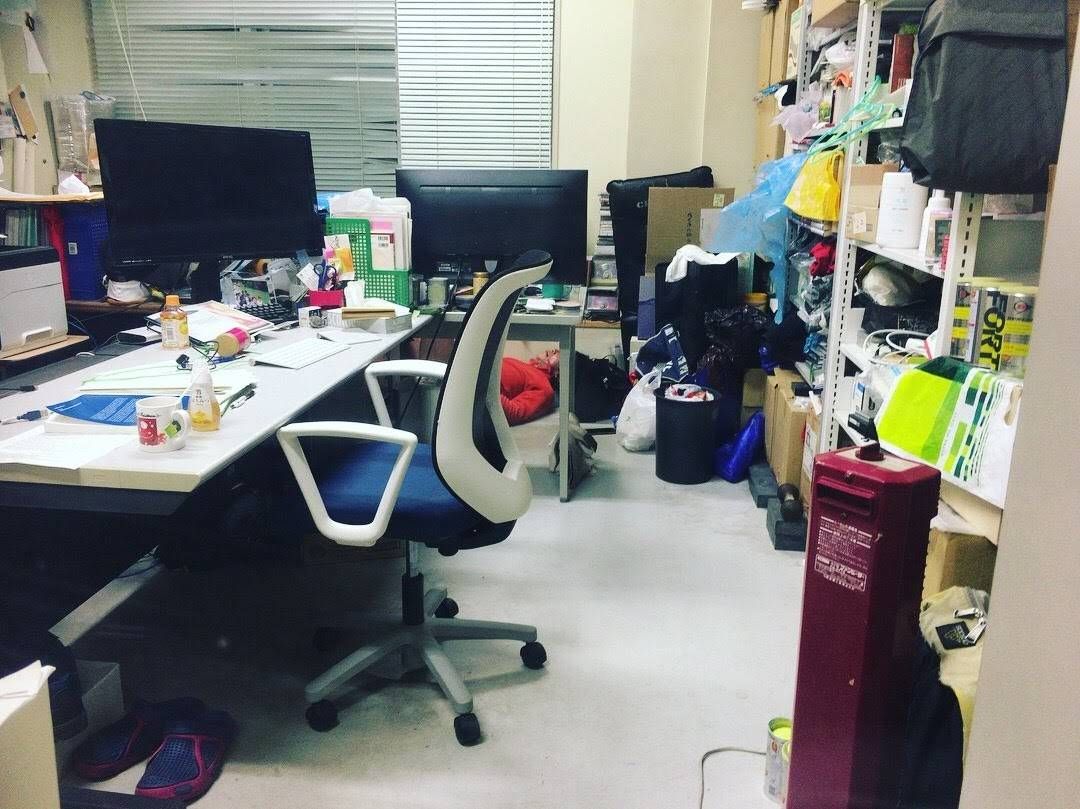
\includegraphics[clip,scale=0.2]{atm1.jpg}
  \caption{こんなことをしているからである。}
\label{atm1}
\end{figure}

\begin{figure}[H]
  \centering
  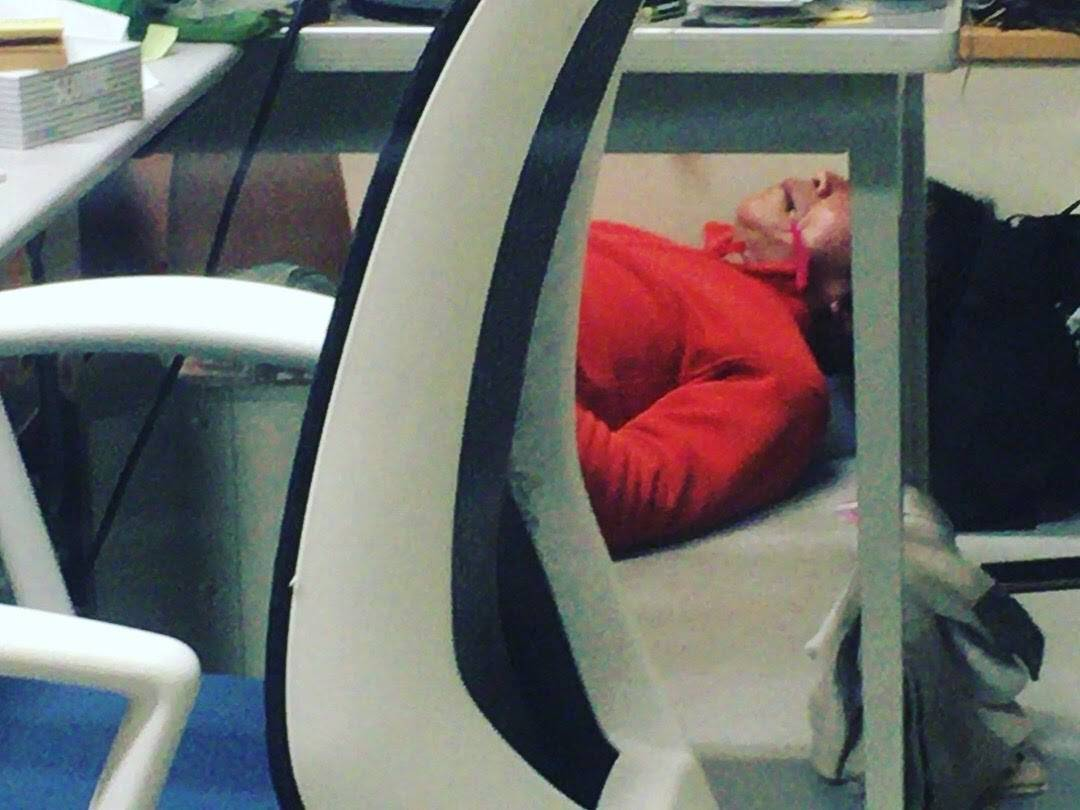
\includegraphics[clip,scale=0.2]{atm2.jpg}
  \caption{撮影者であるティライミ氏曰く「夜中に発見した時はとうとう死んだかと思った」とのこと。}
\label{atm2}
\end{figure}

%~~~~~~~~~~~~~~~~~~~~~~~~~~~~~~~~~~~~~~~~~~~~~~~~~~
\newpage
\section{都留語録}
・(蔵重さんに向かって)次のスライドに書いてるんで安心してください\\
・(蔵重さんに向かって)ごめん\\
・なんちゅう教科書や\\
・えー(蔵重「えーじゃないんですよ」)\\
・ちょっと待ってヒドイ\\
 
12/7\\
・「出張予定ある方、申し上げてください」\\
・「えっーと、山内を消して。。。」\\

\begin{figure}[H]
  \centering
  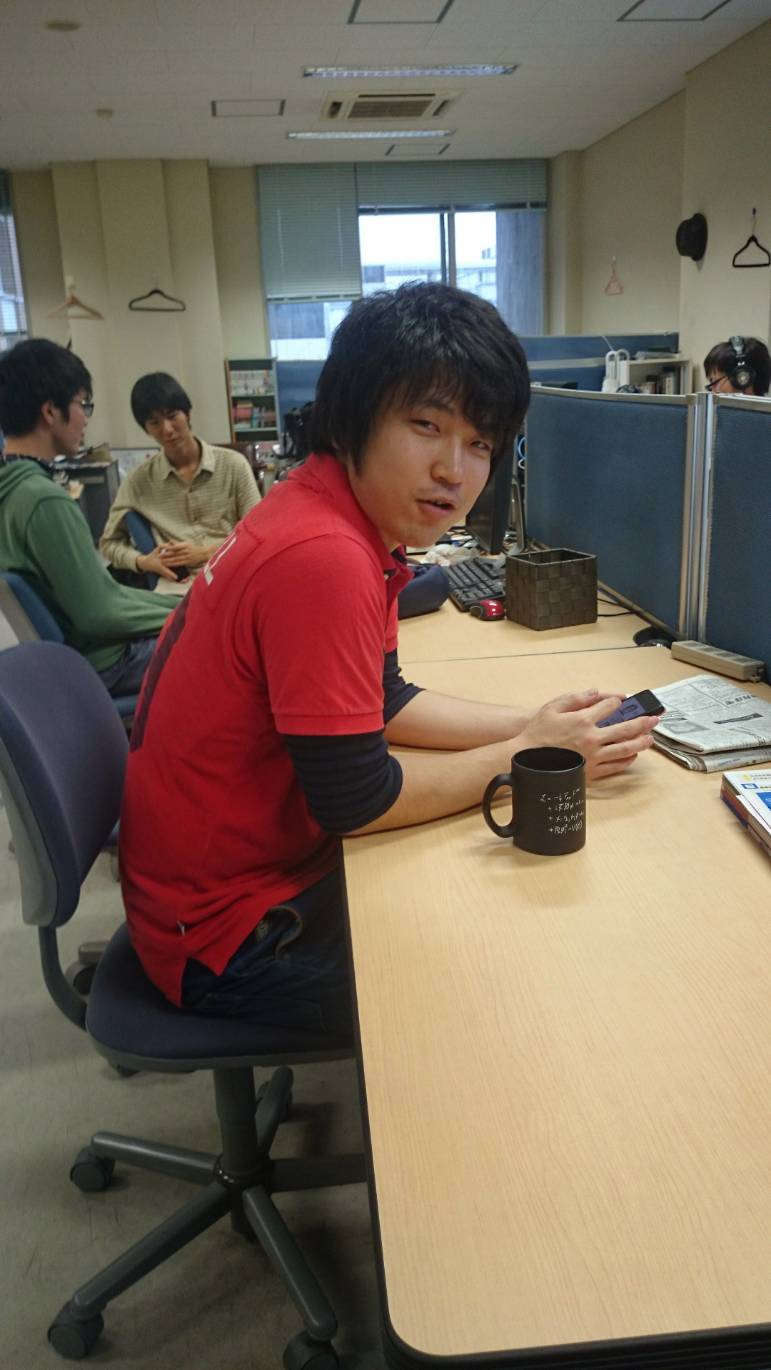
\includegraphics[clip,scale=0.2]{turu.jpg}
  \caption{現存する最古のツルである。}
\label{turu}
\end{figure}
%~~~~~~~~~~~~~~~~~~~~~~~~~~~~~~~~~~~~~~~~~~~~~~~~~~
\newpage
\section{オーキド博士}
これは、いつもいつでもうまくゆくなんて保証はどこにもない、壮大な物語である。\\
 昨今の通信機器の発達により、世界中の至る所でどこでも様々な形式で会話が成立してしまうという緊急事態が生じているといっても過言。まさにバラボンヌである。一方で、その会話の中で、ある種の「当たり前な」発言や、「自明である」状態を指摘される場面は多々あり、それは時事刻々ととめどなく流れている会話の濁流においては淘汰されるべき萃(アツム、と読む。なんか変換で出てきた)のような存在なのである。しかし、そのアツムのような存在を正面から叩き潰すためには現代の技術では不可能に近いため、オーキド博士研究家のアバポン山崎氏(享年0827歳)によって考案されたのが「そらっそうじゃっ」である。\\
 しかし、アバポン山崎氏は現在地球に存在していないため、なぜこのようなオーキド博士の概念が爆誕したのかは不明である(おそらくあくる日の暇カスな日常会話がきっかけであったという説が噂であるらしいが、これはまた別のお話)。\\
以下では、このソラソウジャ並びにオーキド近辺の情報をまとめる。
\subsection{オーキド・ユキナリ}
オーキド・ユキナリは、ゲーム『ポケットモンスター』などに登場する架空の人物。これはオーキド。\\
 また、カントー地方のマサラタウンにある「オーキド研究所」で暮らし、毎日ポケモンを研究している。年齢は55歳で、この点はアツムと類似している。一方で、多少変人扱いされているらしいが、マサラタウンの住人達から慕われているらしい。この点はアツムとは正反対である。\\
 そして、孫の姉弟がおり弟の方は『赤・緑』『ファイアレッド・リーフグリーン』で全人類のライバルとなる。姉の名前はナナミで、ブリーダーとしてかなりの腕があるらしい。したがって孫の存在から既婚になるが、妻や子は現在までに一切登場していない。この点もアツムと類似している。\\
 以上より、オーキドの正体は誤差の範囲内でアツムであると言える。

\subsection{岡山県総社駅}
アバポン山崎氏が死に際、長々と語った話を総合すると、オーキドとオガワ・インティ・ライミ氏は深い関係があるらしい。要約すると以下の通りである。\\
 ある日、岡山県の倉敷のアウトレット(図\ref{kurashiki})に出かけたオガワ・インティ・ライミ氏は、平成30年7月豪雨の影響で在来線が運休し、家の最寄駅まで代行バスで行く必要があった。しかし長距離であるため、とある駅でまたバスを乗り換えるという事態が生じた。その駅こそが伝説の「総社駅」である(図\ref{soja1})。しかも驚くことに、駅名標のとなりの広告にはオガワ・インティ・ライミ公式ドリンクの「カルピス」が掲載されていたのである(図\ref{soja2})。

\begin{figure}[H]
\centering
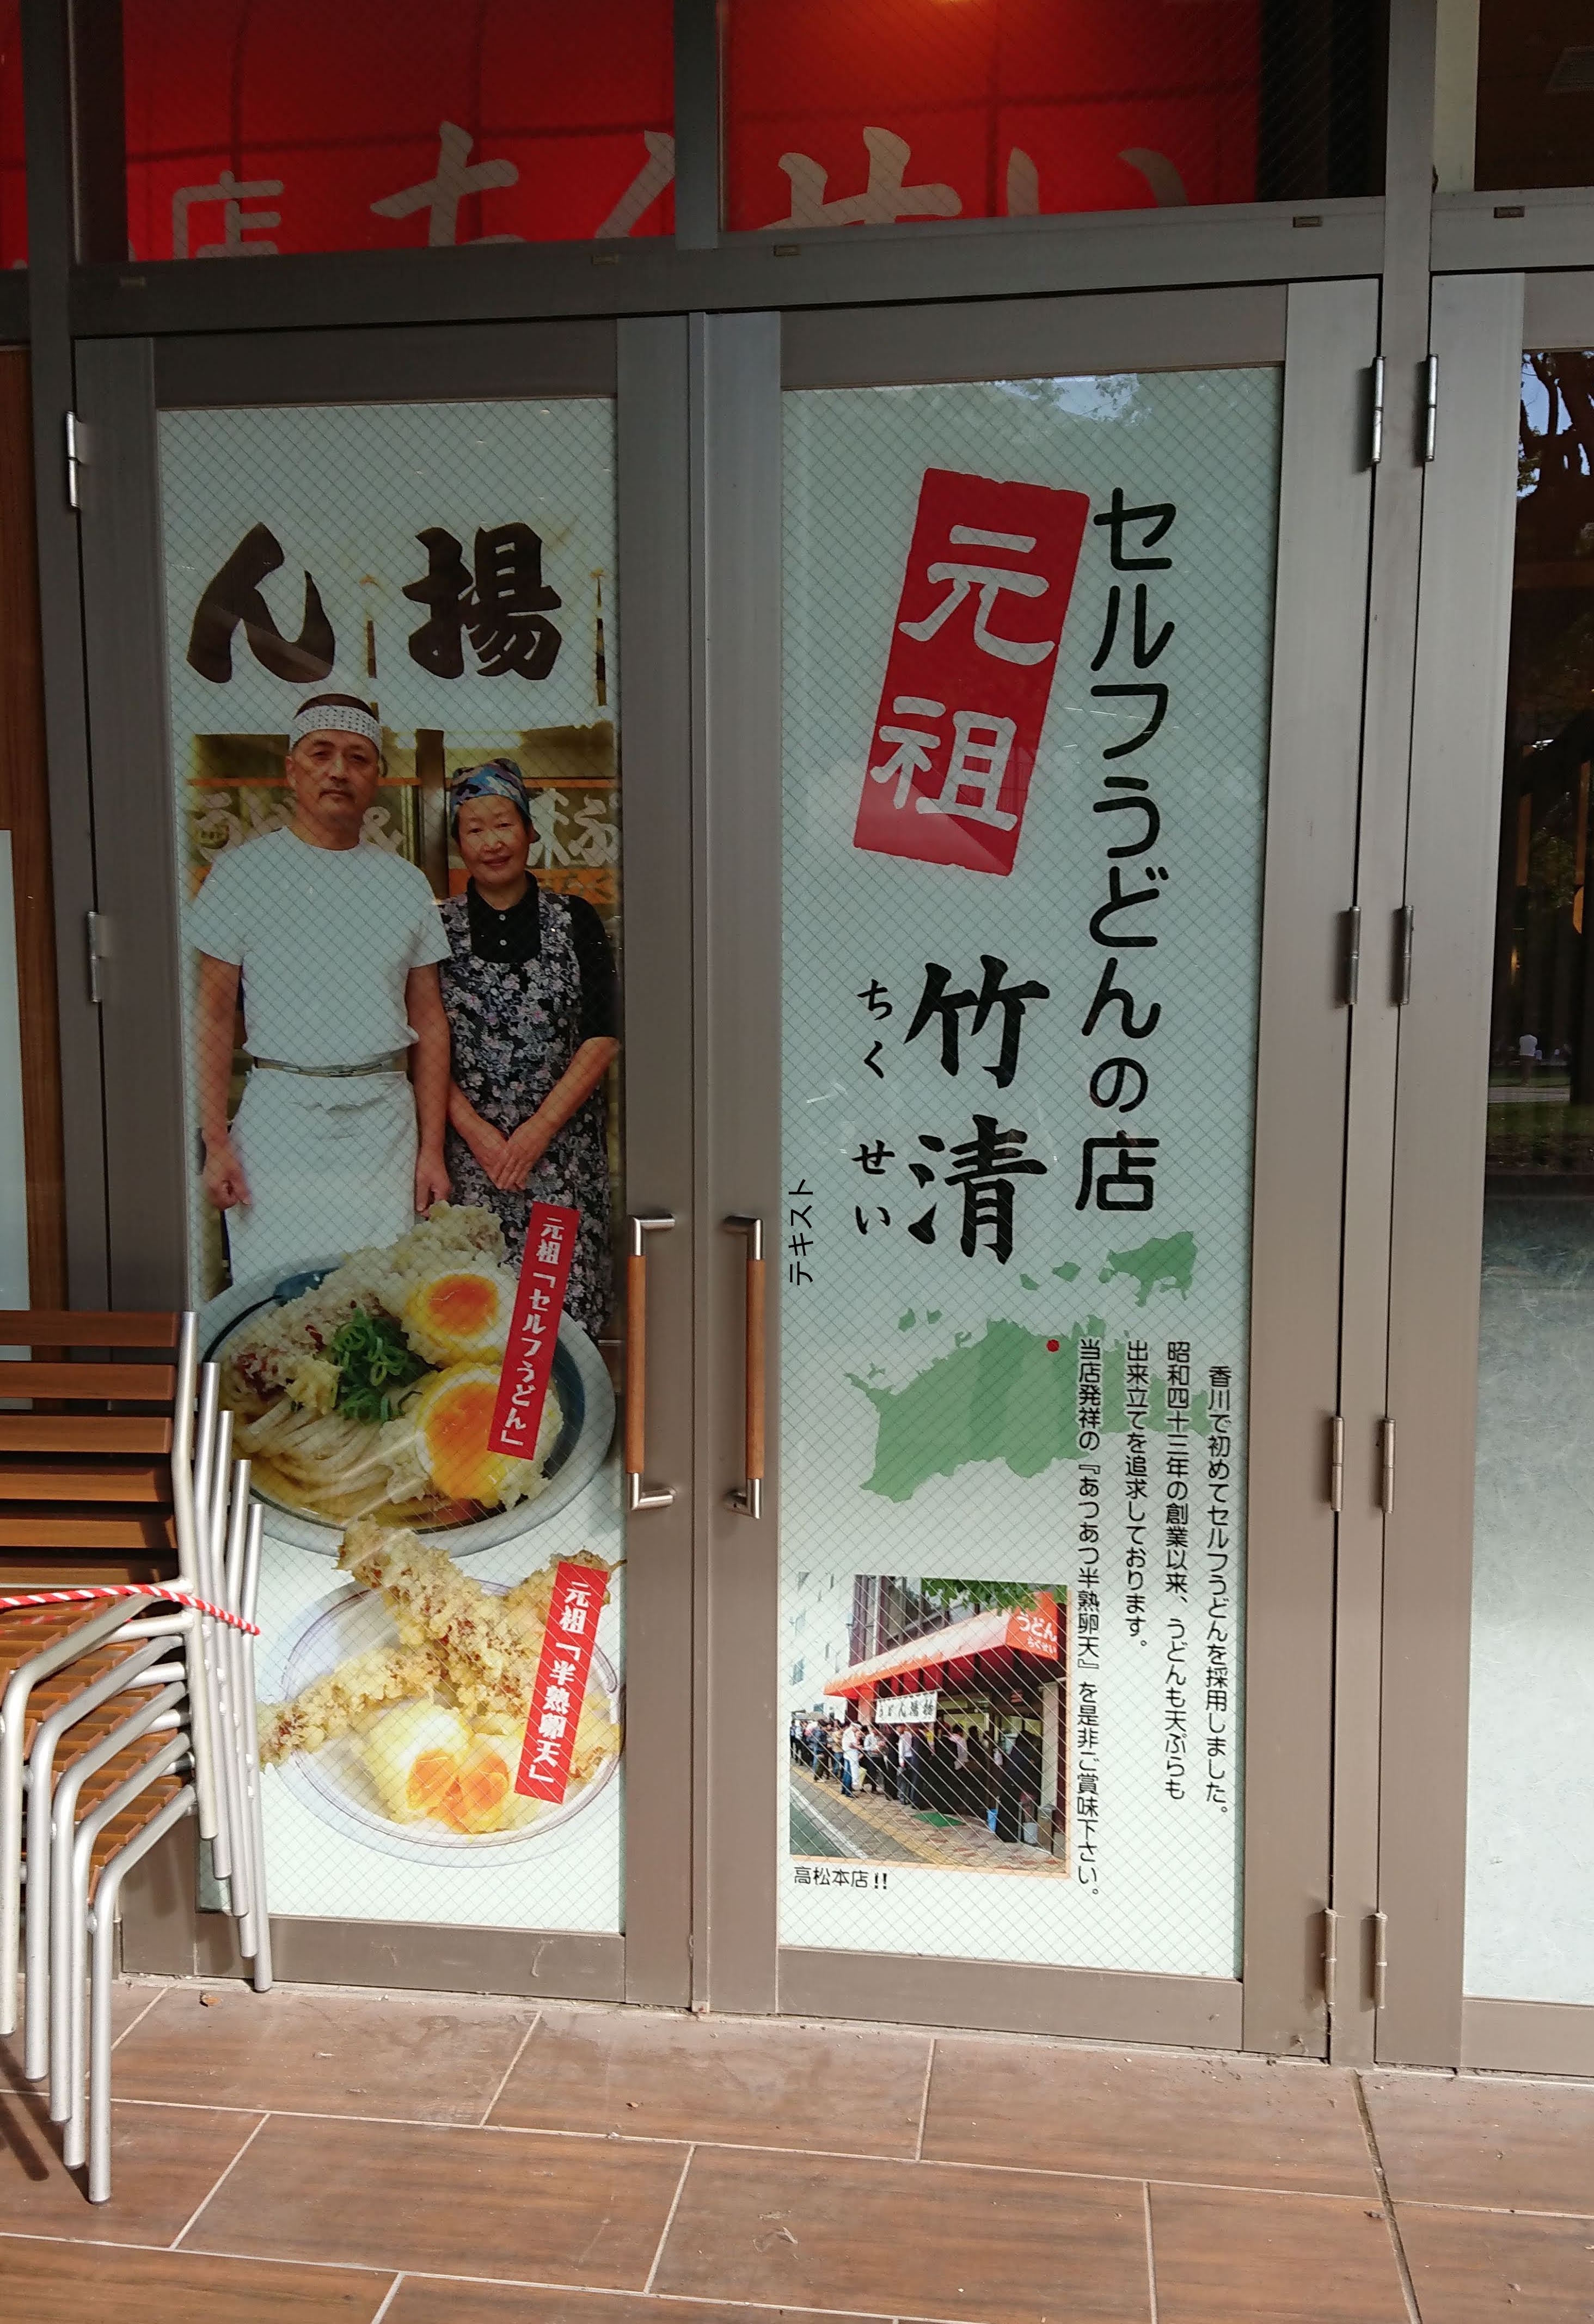
\includegraphics[scale=0.05]{kurashiki.jpg}
\caption{倉敷のアウトレットにあった元祖セルフうどんの店「竹清」。よく考えたら学部の頃に行った香川うどん踊り食い旅行のときになんかあったような。まあそんなことより「竹」という字から、ここもタケダ氏の支配下に置かれていることがうかがえる。}
\label{kurashiki}
\end{figure}


\begin{figure}[htbp]
 \begin{minipage}{0.4\hsize}
  \begin{center}
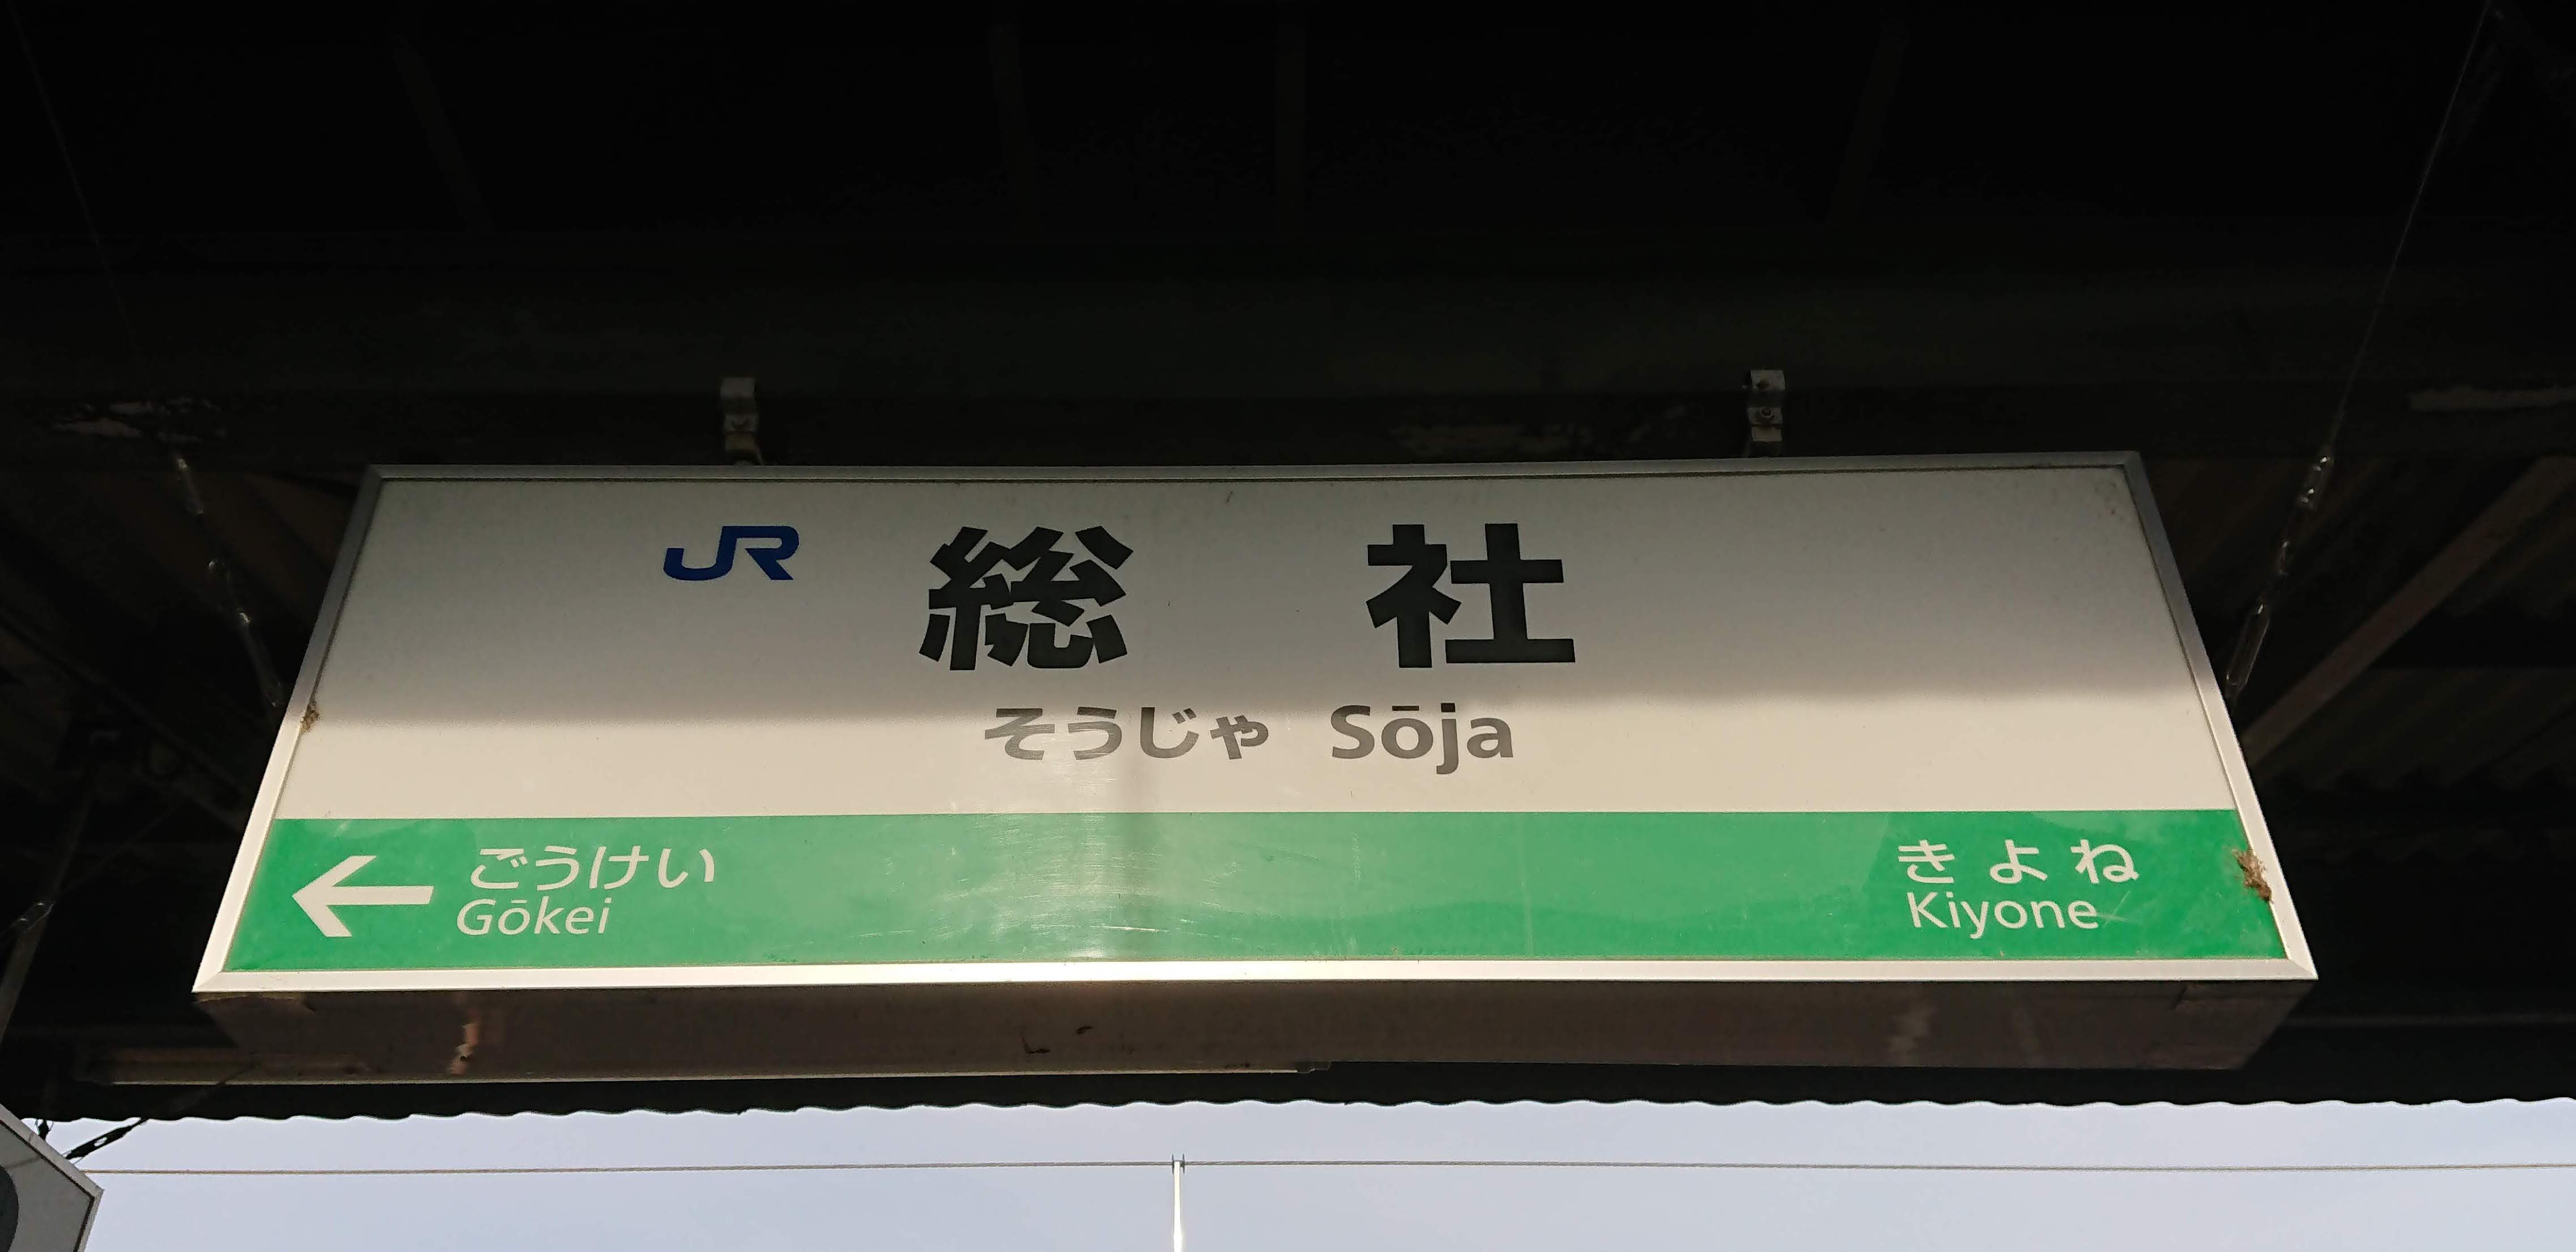
\includegraphics[width=1\textwidth]{soja1.jpg}
  \end{center}
  \label{soja1}
 \end{minipage}
 \begin{minipage}{0.4\hsize}
  \begin{center}
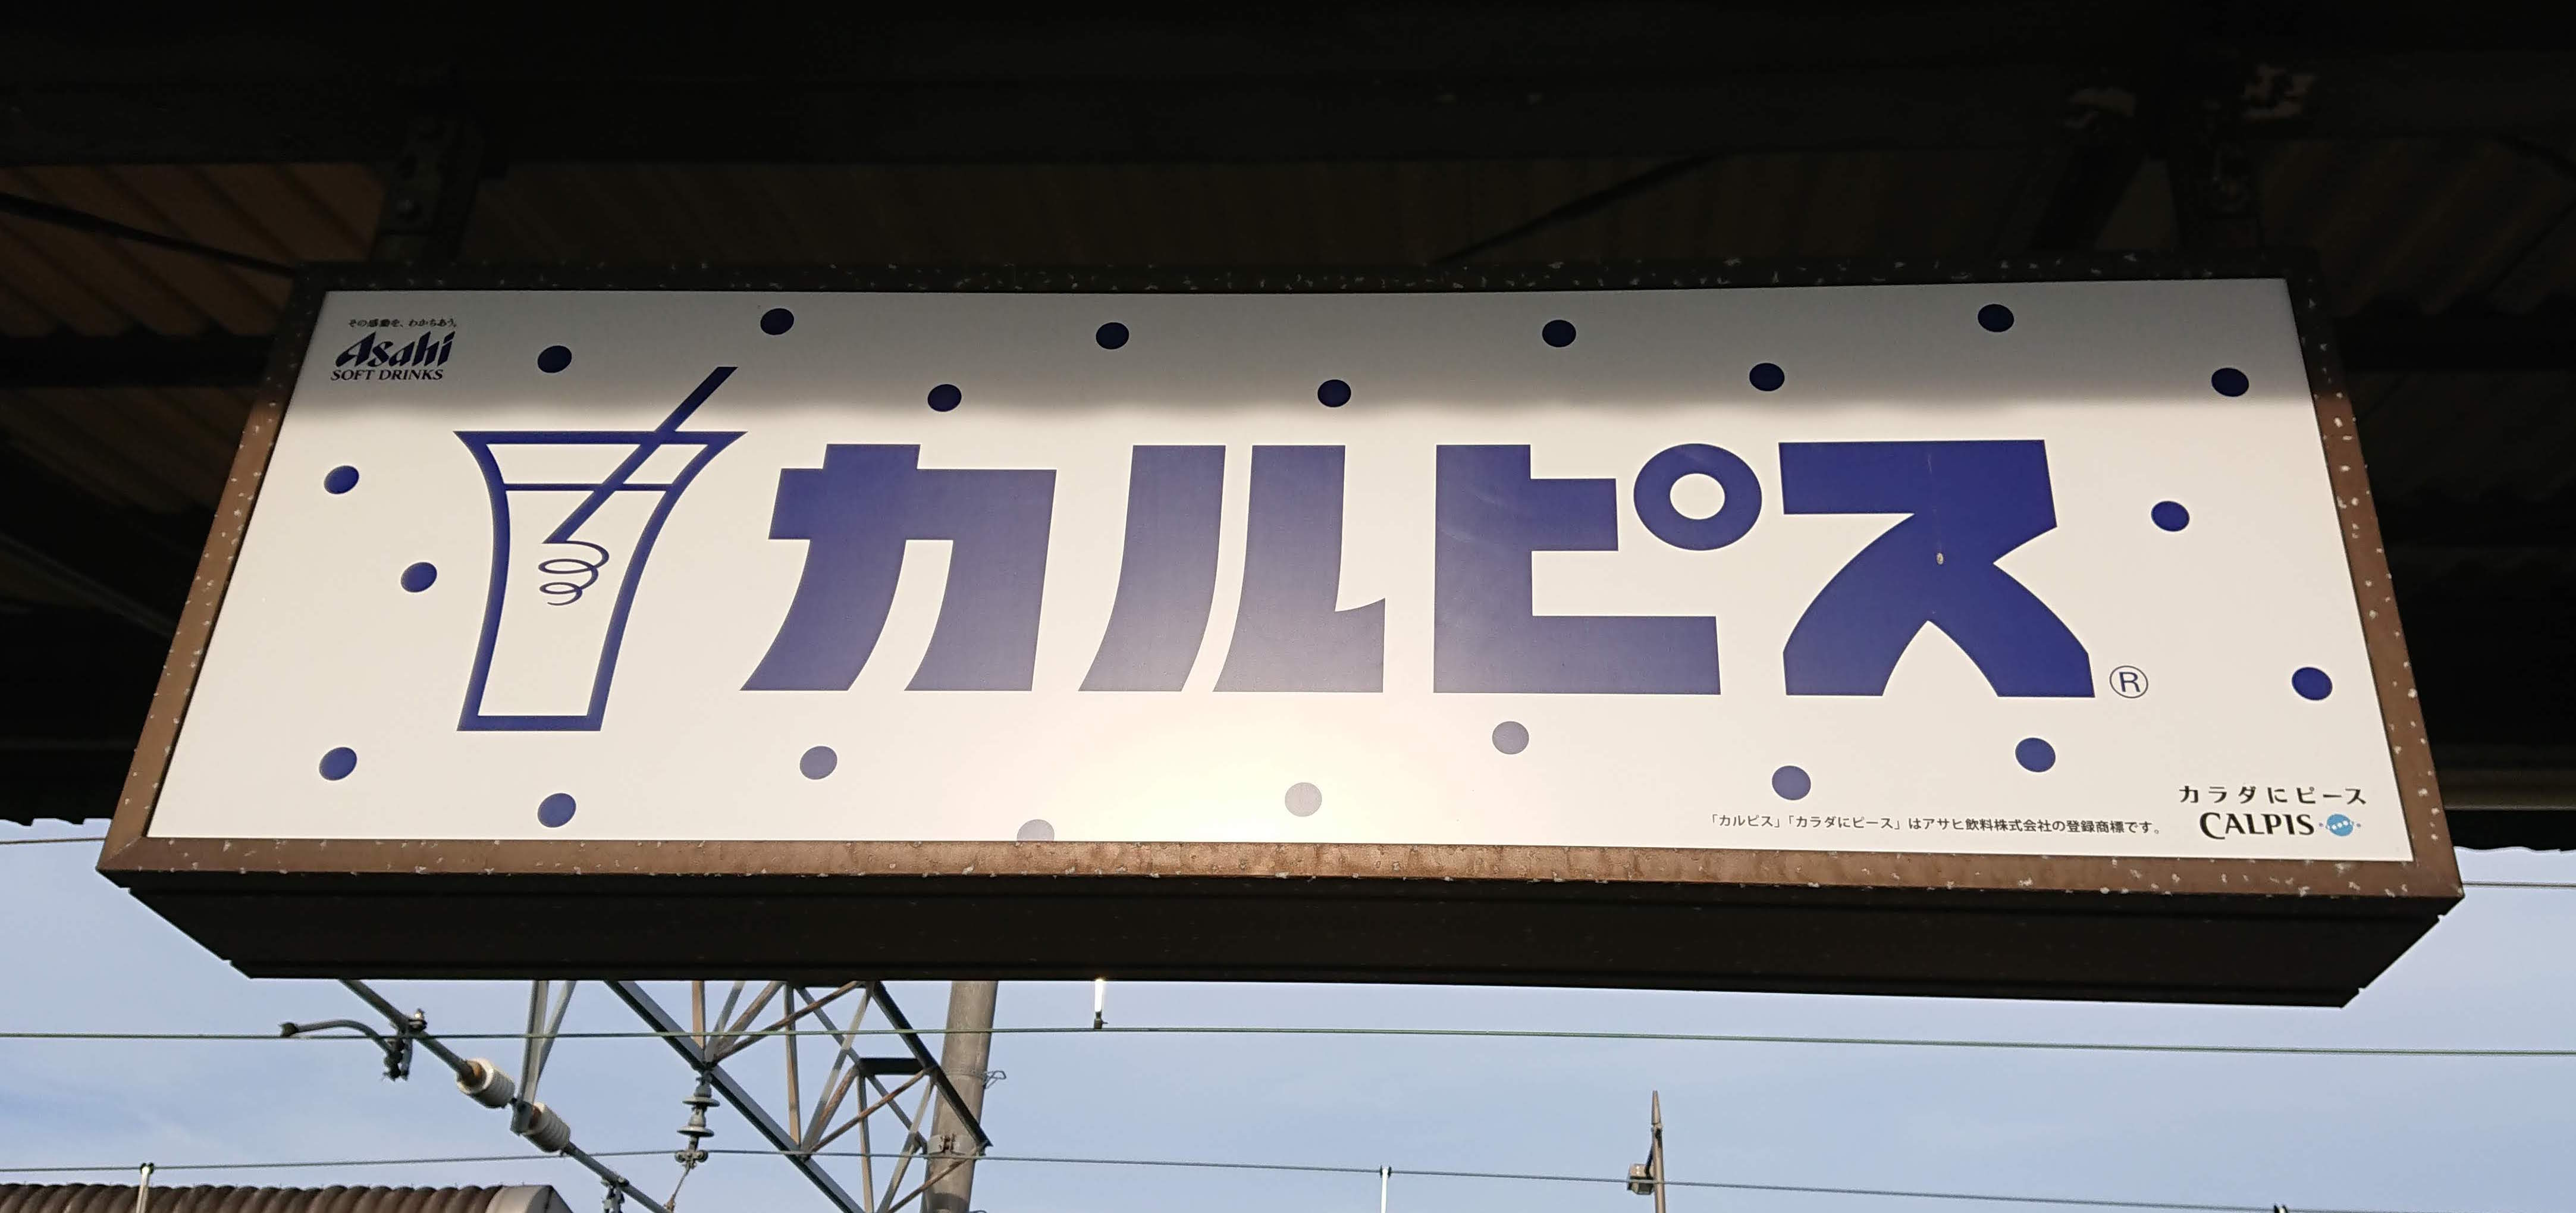
\includegraphics[width=1\textwidth]{soja2.jpg}
  \end{center}
 \end{minipage}
 \caption{総社駅とカルピス。そらそうじゃと言わんばかりである。}
  \label{soja2}
\end{figure}

\subsection{今後の展望}
このオーキドという概念は、大学の時のノリのまま封印されるというのが大方の予想であった。しかし、2018年のいつか忘れたけど、衝撃的なニュースが宇宙中を震撼させた。「オーキド博士死亡」である(図\ref{ookidosibou})。

\begin{figure}[H]
\centering
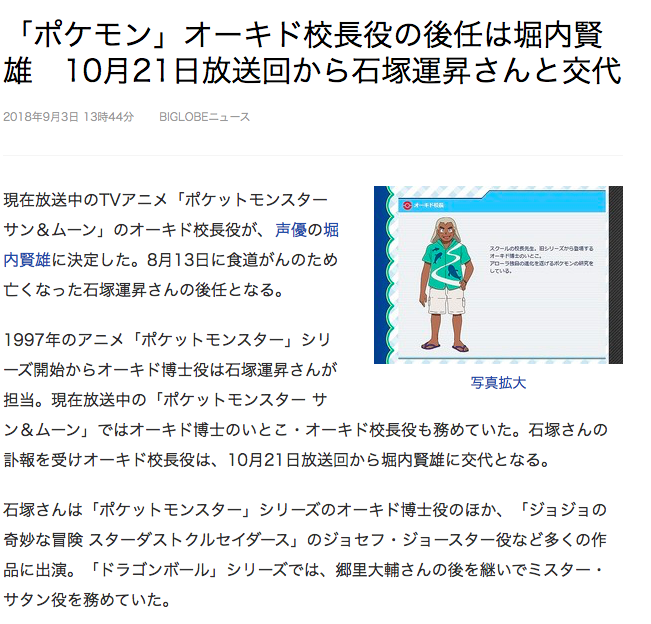
\includegraphics[scale=0.25]{ookidosibou.png}
\caption{誰やねん}
\label{ookidosibou}
\end{figure}

この瞬間から急激なオオキドの減少という人類の危機に迫られていた矢先、奇跡は起こったのである。\\
 衝撃ニュースを流すべく、オガワ・インティ・ライミが新入社員研修で同部屋だった仲の良い同期とのLINEグループに投下すると、即座にオーキド完全体が爆誕したのである(図\ref{sora})。これはまさに、社会人として遠く離れた地静岡に乗り込みながらも、地道なオーキド普及活動を行ってきた賜物であり、今後も世界中がオーキドの息の根を止めさせず、永遠に語り継がれる何かになると言っても過言。そらっっっっっっっっっっっっっ

\begin{figure}[H]
\centering
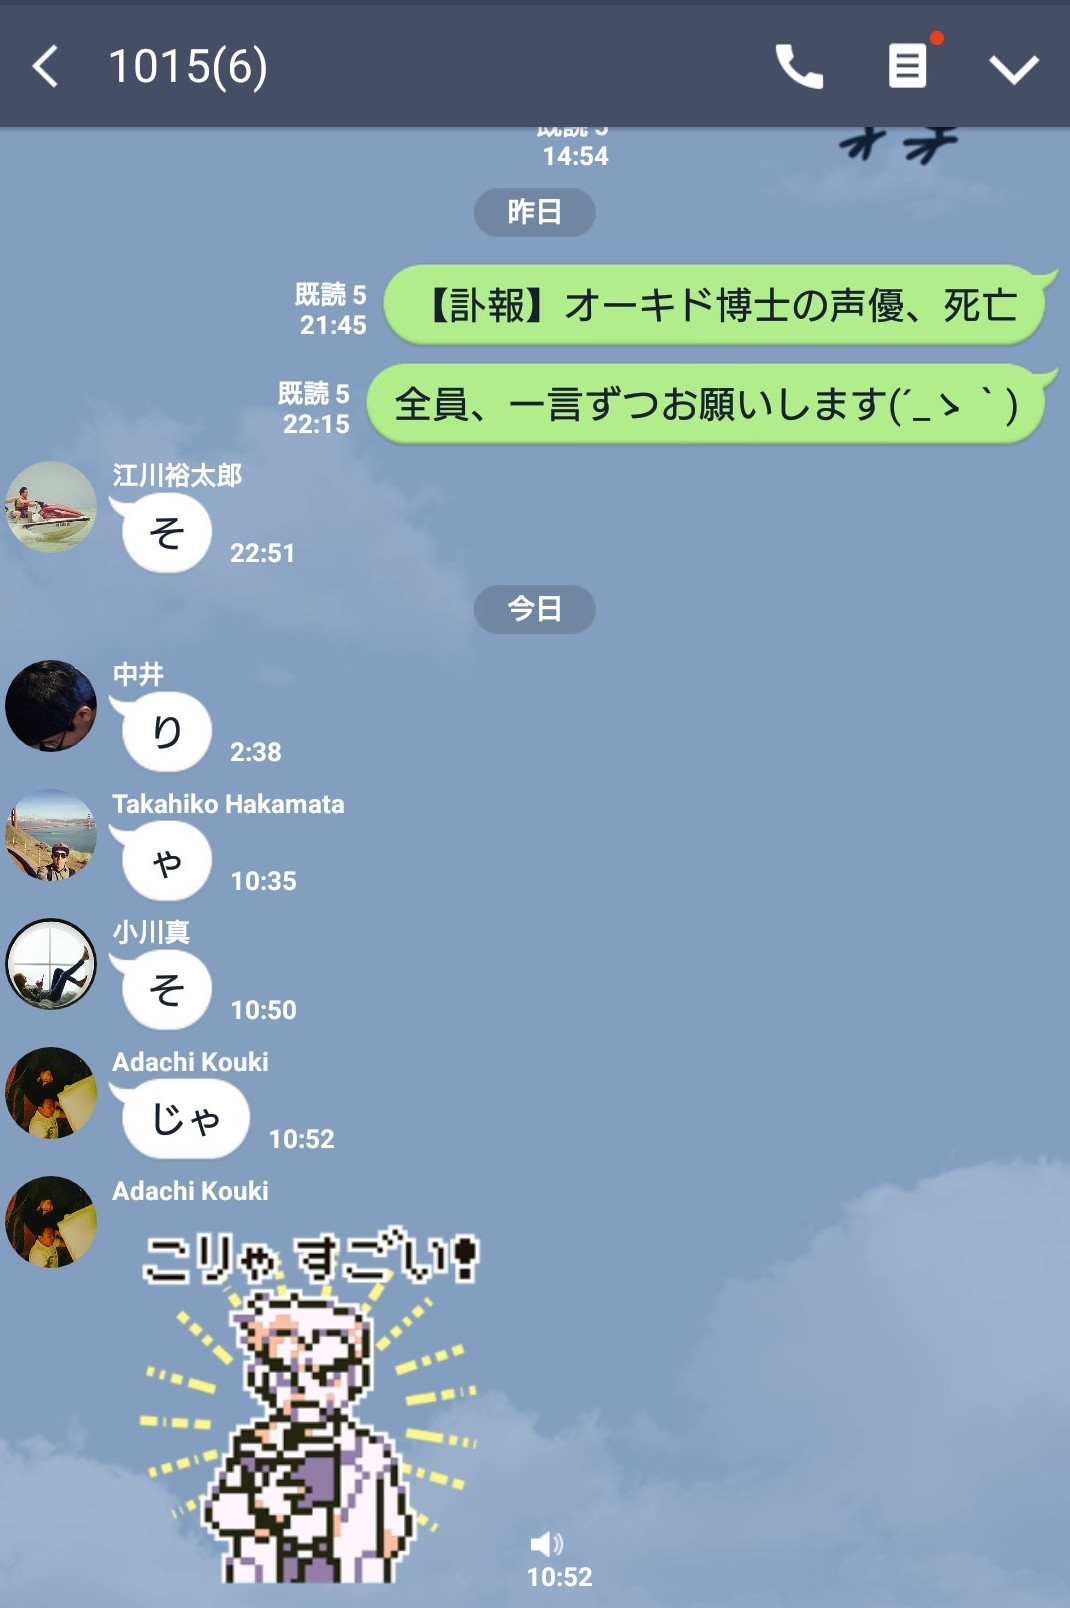
\includegraphics[scale=0.15]{sora.jpg}
\caption{会話自体はこれで終了という、もはや重症患者}
\label{sora}
\end{figure}

%~~~~~~~~~~~~~~~~~~~~~~~~~~~~~~~~~~~~~~~~~~~~~~~~~~
\newpage
\section{広告}
\subsubsection{オガワ・インティ・ライミ 詩集}
数々の楽曲を提供してきたオガワ・インティ・ライミ。\\
この度詩集を発表することとなりました。\\
青春時代を生きるすべての老若男女に捧ぐ、愛の鎮魂歌。詩集のタイトルは\\
 \\
「希望新風\UTF{FF5E}明日への道\UTF{FF5E}」\\
 \\
希望に満ち、将来の不安に怯えながらも自らの人生に新しい風"新風"を吹き込む助けになる詩集を目指し、執筆したとのことです。(集英社/¥1050)\\
この詩集「希望新風\UTF{FF5E}明日への道\UTF{FF5E}」には延べ3万ものポエムが綴られていますが、その中でも選りすぐりの詩を、まだ本書を手にしていない貴方へ送ります。\\
きっと明日への道が開かれんことを。\\
この詩を読んで感銘を受けた方は是非、本書の購入の検討を...!\\
 \\
""未来の自分へ(本書p3560  第2章冒頭部)""\\
(shiny)希望新風からのお知らせ(shiny)\\
 \\
(えへへ)塩油そば終了です(Moon satisfied)\\
ご来店ありがとうございました(ナイス)\\
次回のサービスにご期待くださいね(えへへ)またのお越しをお待ちしております(ナイス)\\
 \\
""人間合格(本書p5680  第2章中盤)""\\
(shiny)11月1日限定(!)\\
希望新風神戸灘店からのお知らせ(shiny)\\
 \\
おはようございます(ぎゃはは)\\
今日は寒いですね\UTF{FF5E}(Moon satisfied)(Moon satisfied)こんな時は希望新風で暖まりましょう(ナイス)\\
という事で本日のサービスは、、塩油そば(!!!)を500 円でご提供させて頂きます(Chef)ご注文の際にこの画面をお見せください(ナイス)\\
限定商品の為、売り切れ次第終了とさせて頂きます(おねがい)この機会に是非、希望新風にお越しくださいませ(えへへ)\\

%~~~~~~~~~~~~~~~~~~~~~~~~~~~~~~~~~~~~~~~~~~~~~~~~~~
\newpage
\section{蔵重警察の不法行為一覧}
\subsection{竹田食堂閉店事件}
11/17に発生した職権濫用の代表的な事件。年の瀬も近付いてきた頃に、それまで地元で永らく愛されてきた竹田食堂の閉店を迫った。店主は反発するも、何の事情の説明も無いまま閉店へと追いやられた(図\ref{ramentakeda})。\\
現時点で最高裁までもつれこみ、来年度中にも判決が出る模様。今のところ、竹田食堂側が圧倒的に不利であるらしい。
\subsection{騒音事件}
住居から爆音で垂れ流している日本文楽や能などのお囃子にまつわる事件。\\
97年、最高裁判決 蔵重敗訴。

\subsection{衝突事件}
生徒が主軸であるゼミ形式の授業において、とある准教授に向けて知識を問う場面が多々あり意見を准教授とぶつけあうという有名な事件。\\
98年、地方裁判決 死刑。

\begin{figure}[H]
\centering
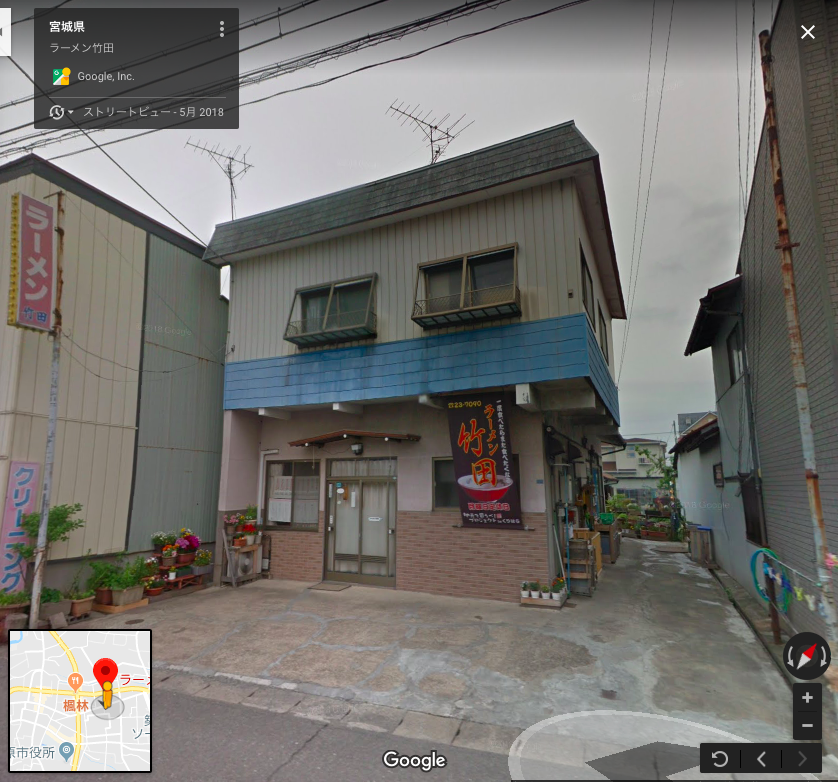
\includegraphics[scale=0.3]{ramentakeda.png}
\caption{ラーメン竹田という実在する店。オガワ・インティ・ライミ氏が宮城県に研修で訪れる際の宿泊施設の近くに存在するという。宮城県栗原市築館伊豆1丁目8−45。}
\label{ramentakeda}
\end{figure}


%~~~~~~~~~~~~~~~~~~~~~~~~~~~~~~~~~~~~~~~~~~~~~~~~~~
\newpage
\section{内閣発足}

\begin{figure}[H]
\centering
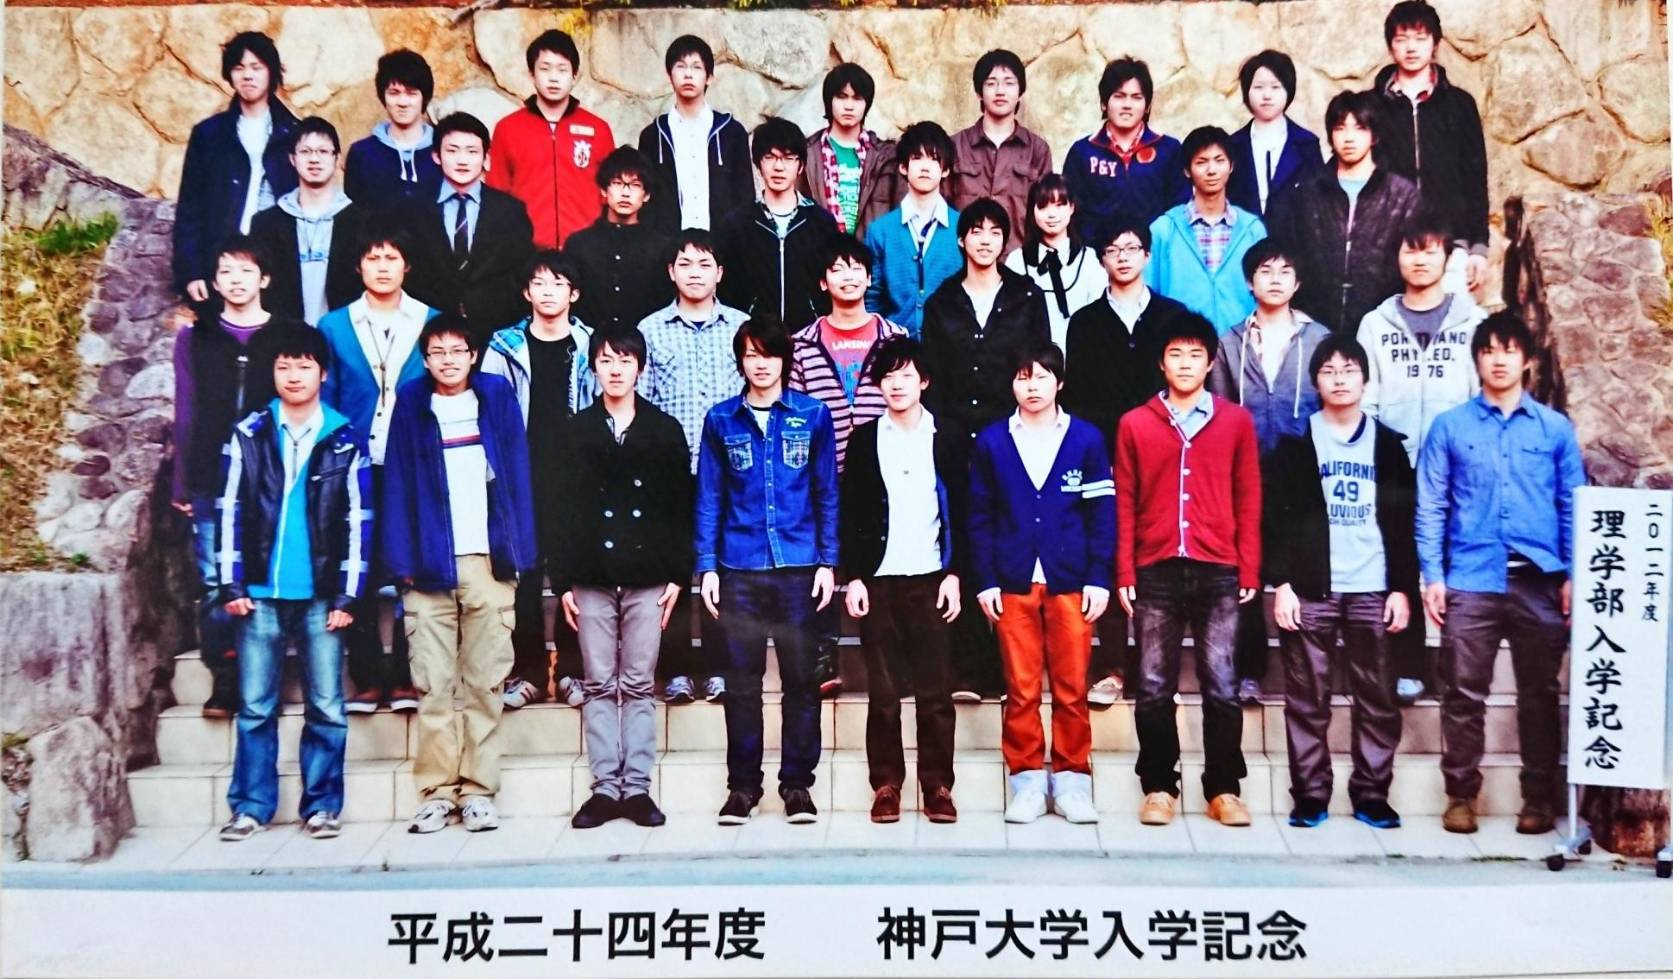
\includegraphics[scale=0.25]{na1}
\caption{第1次内閣}
\label{na1}
\end{figure}

\begin{figure}[H]
\centering
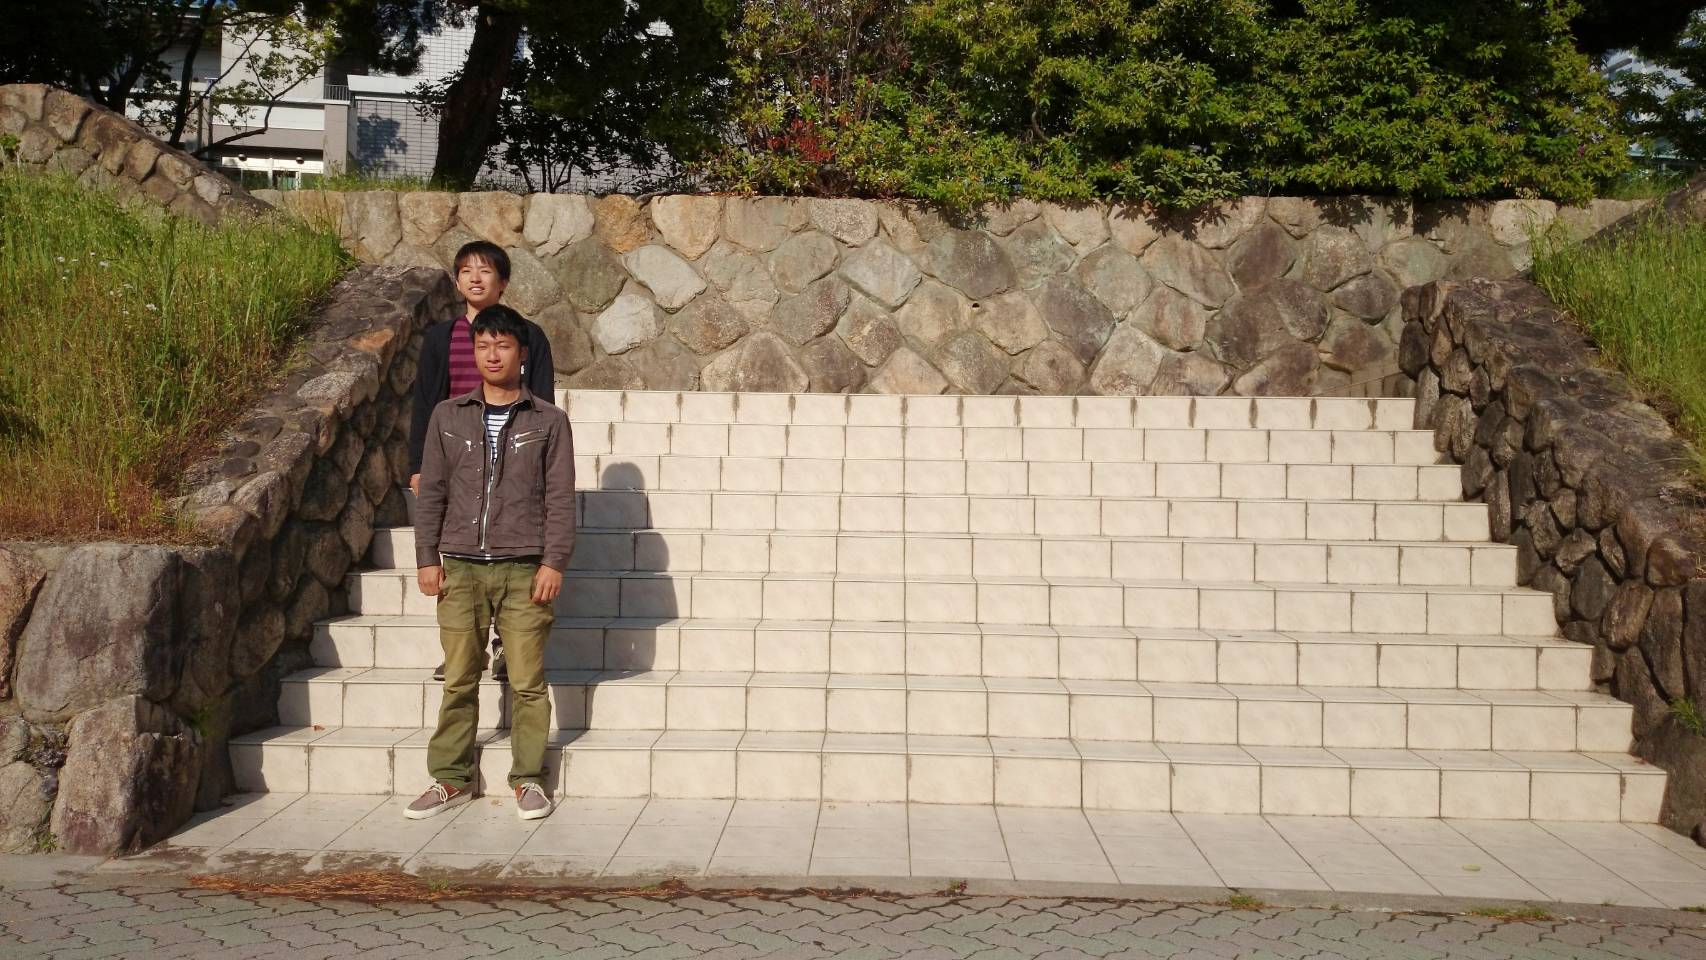
\includegraphics[scale=0.25]{na2}
\caption{第2次内閣}
\label{na2}
\end{figure}

\begin{figure}[H]
\centering
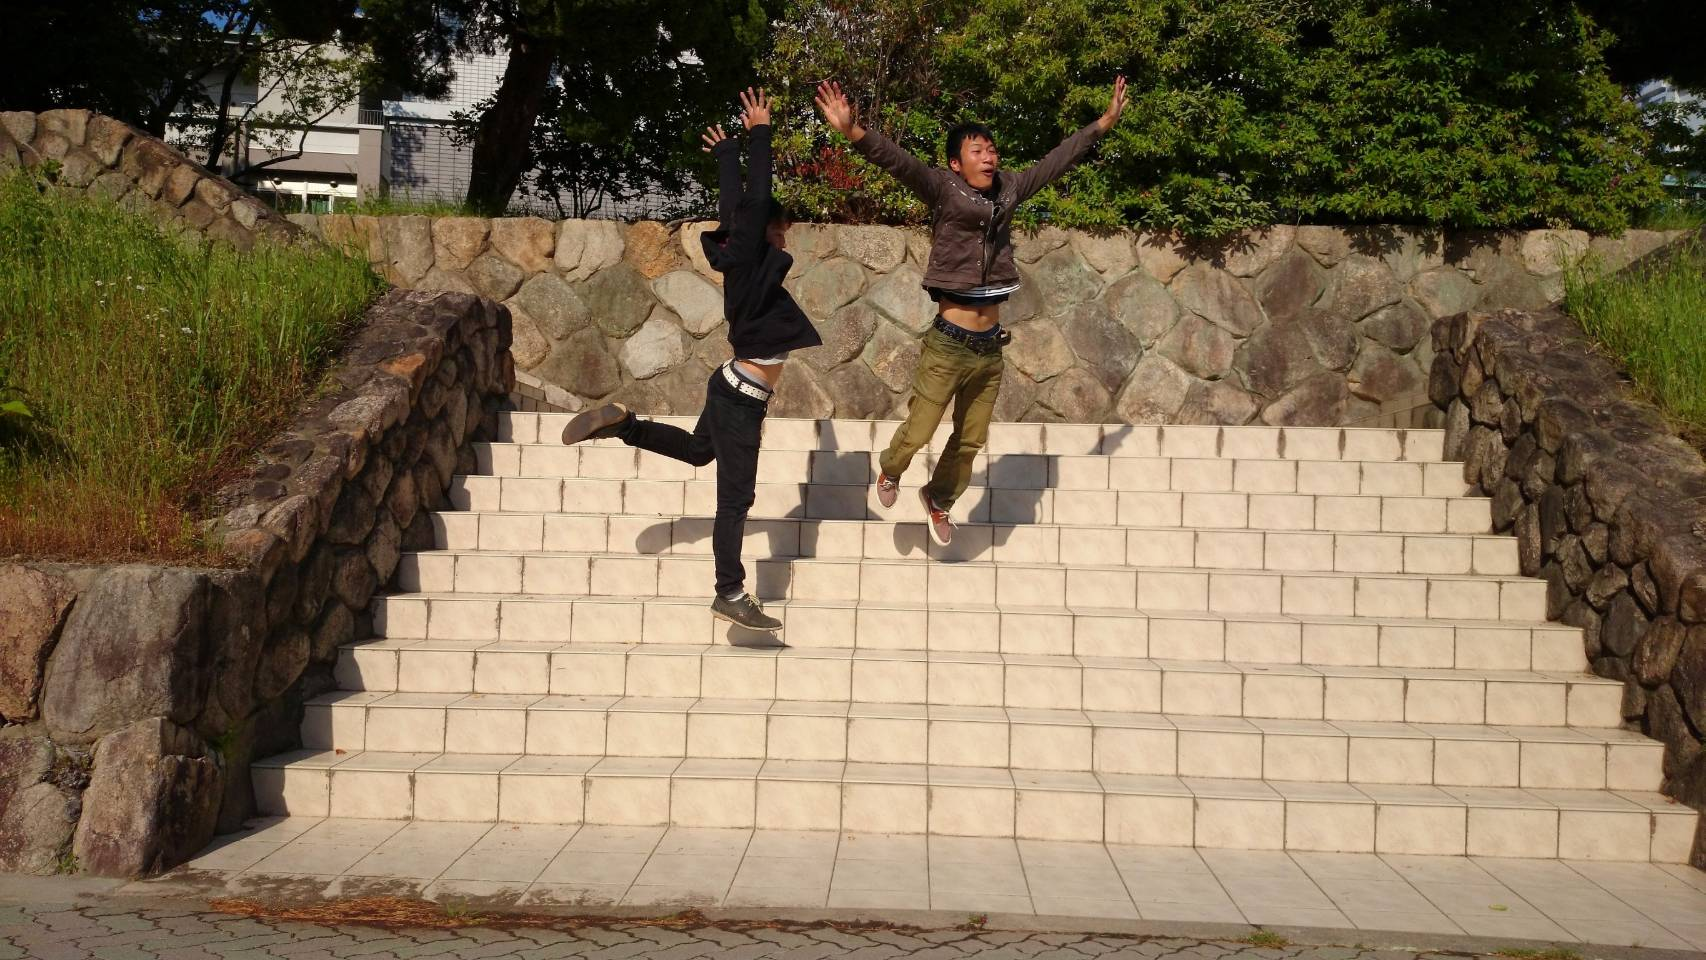
\includegraphics[scale=0.25]{na3}
\caption{第3次内閣}
\label{na3}
\end{figure}

\begin{figure}[H]
\centering
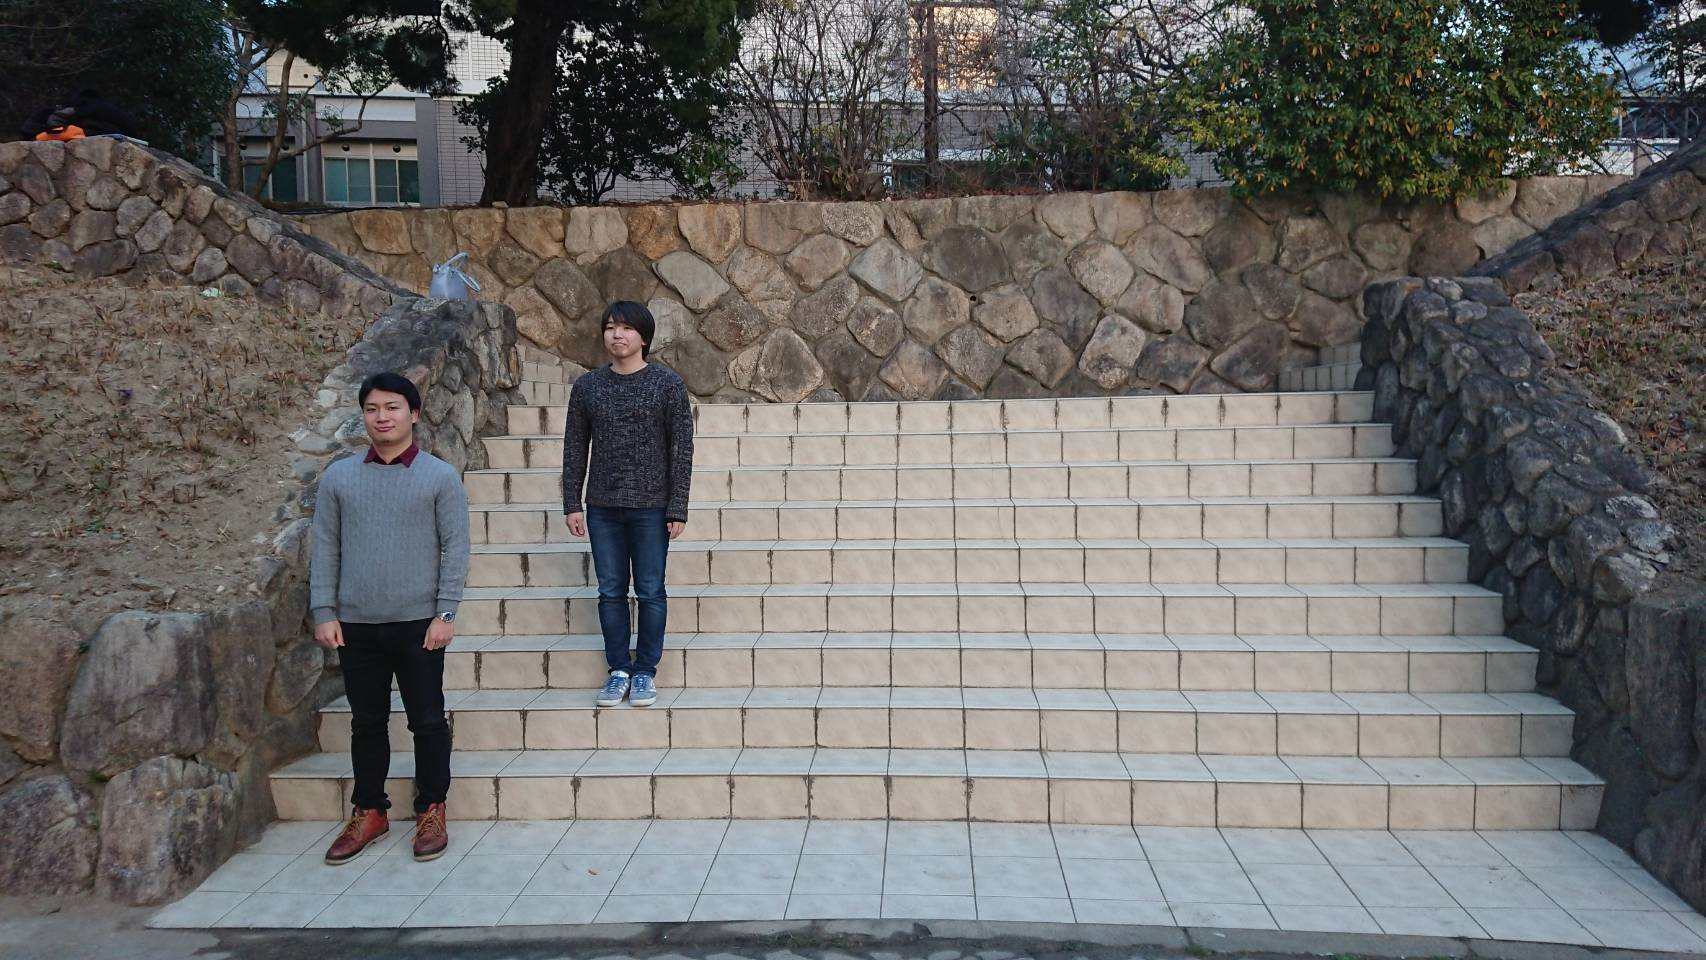
\includegraphics[scale=0.25]{na4}
\caption{第4次内閣}
\label{na4}
\end{figure}

\begin{figure}[H]
\centering
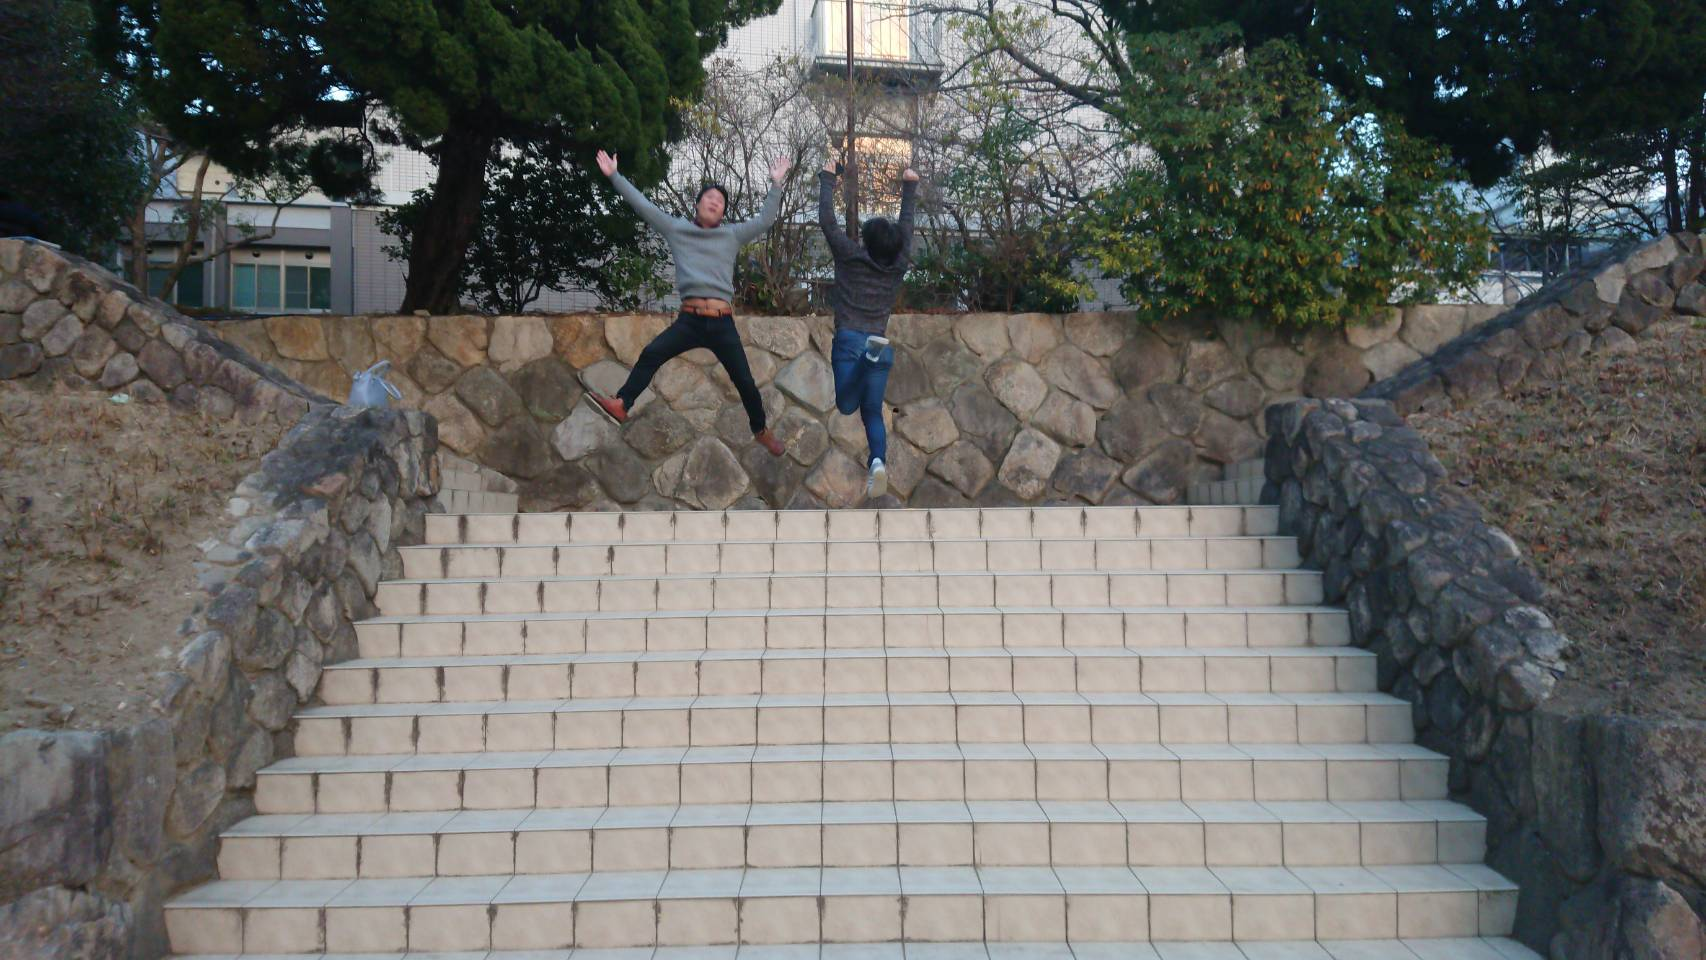
\includegraphics[scale=0.25]{na5}
\caption{第5次内閣}
\label{na5}
\end{figure}

\begin{figure}[H]
\centering
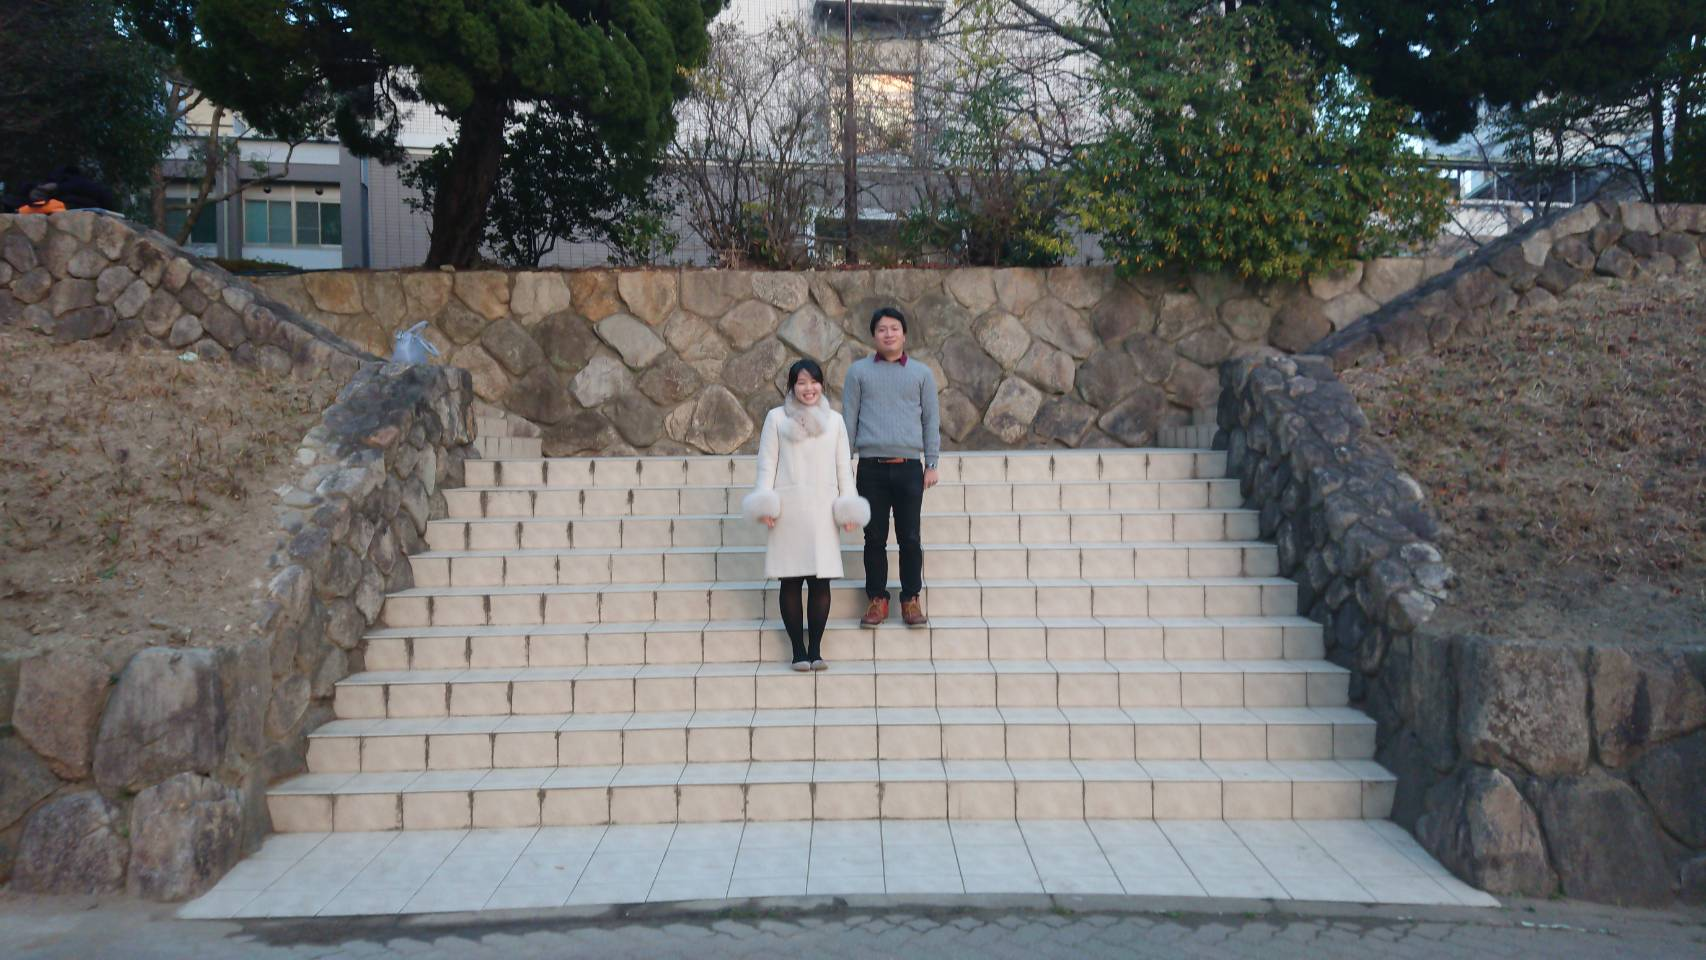
\includegraphics[scale=0.25]{na6}
\caption{第6次内閣}
\label{na6}
\end{figure}

\begin{figure}[H]
\centering
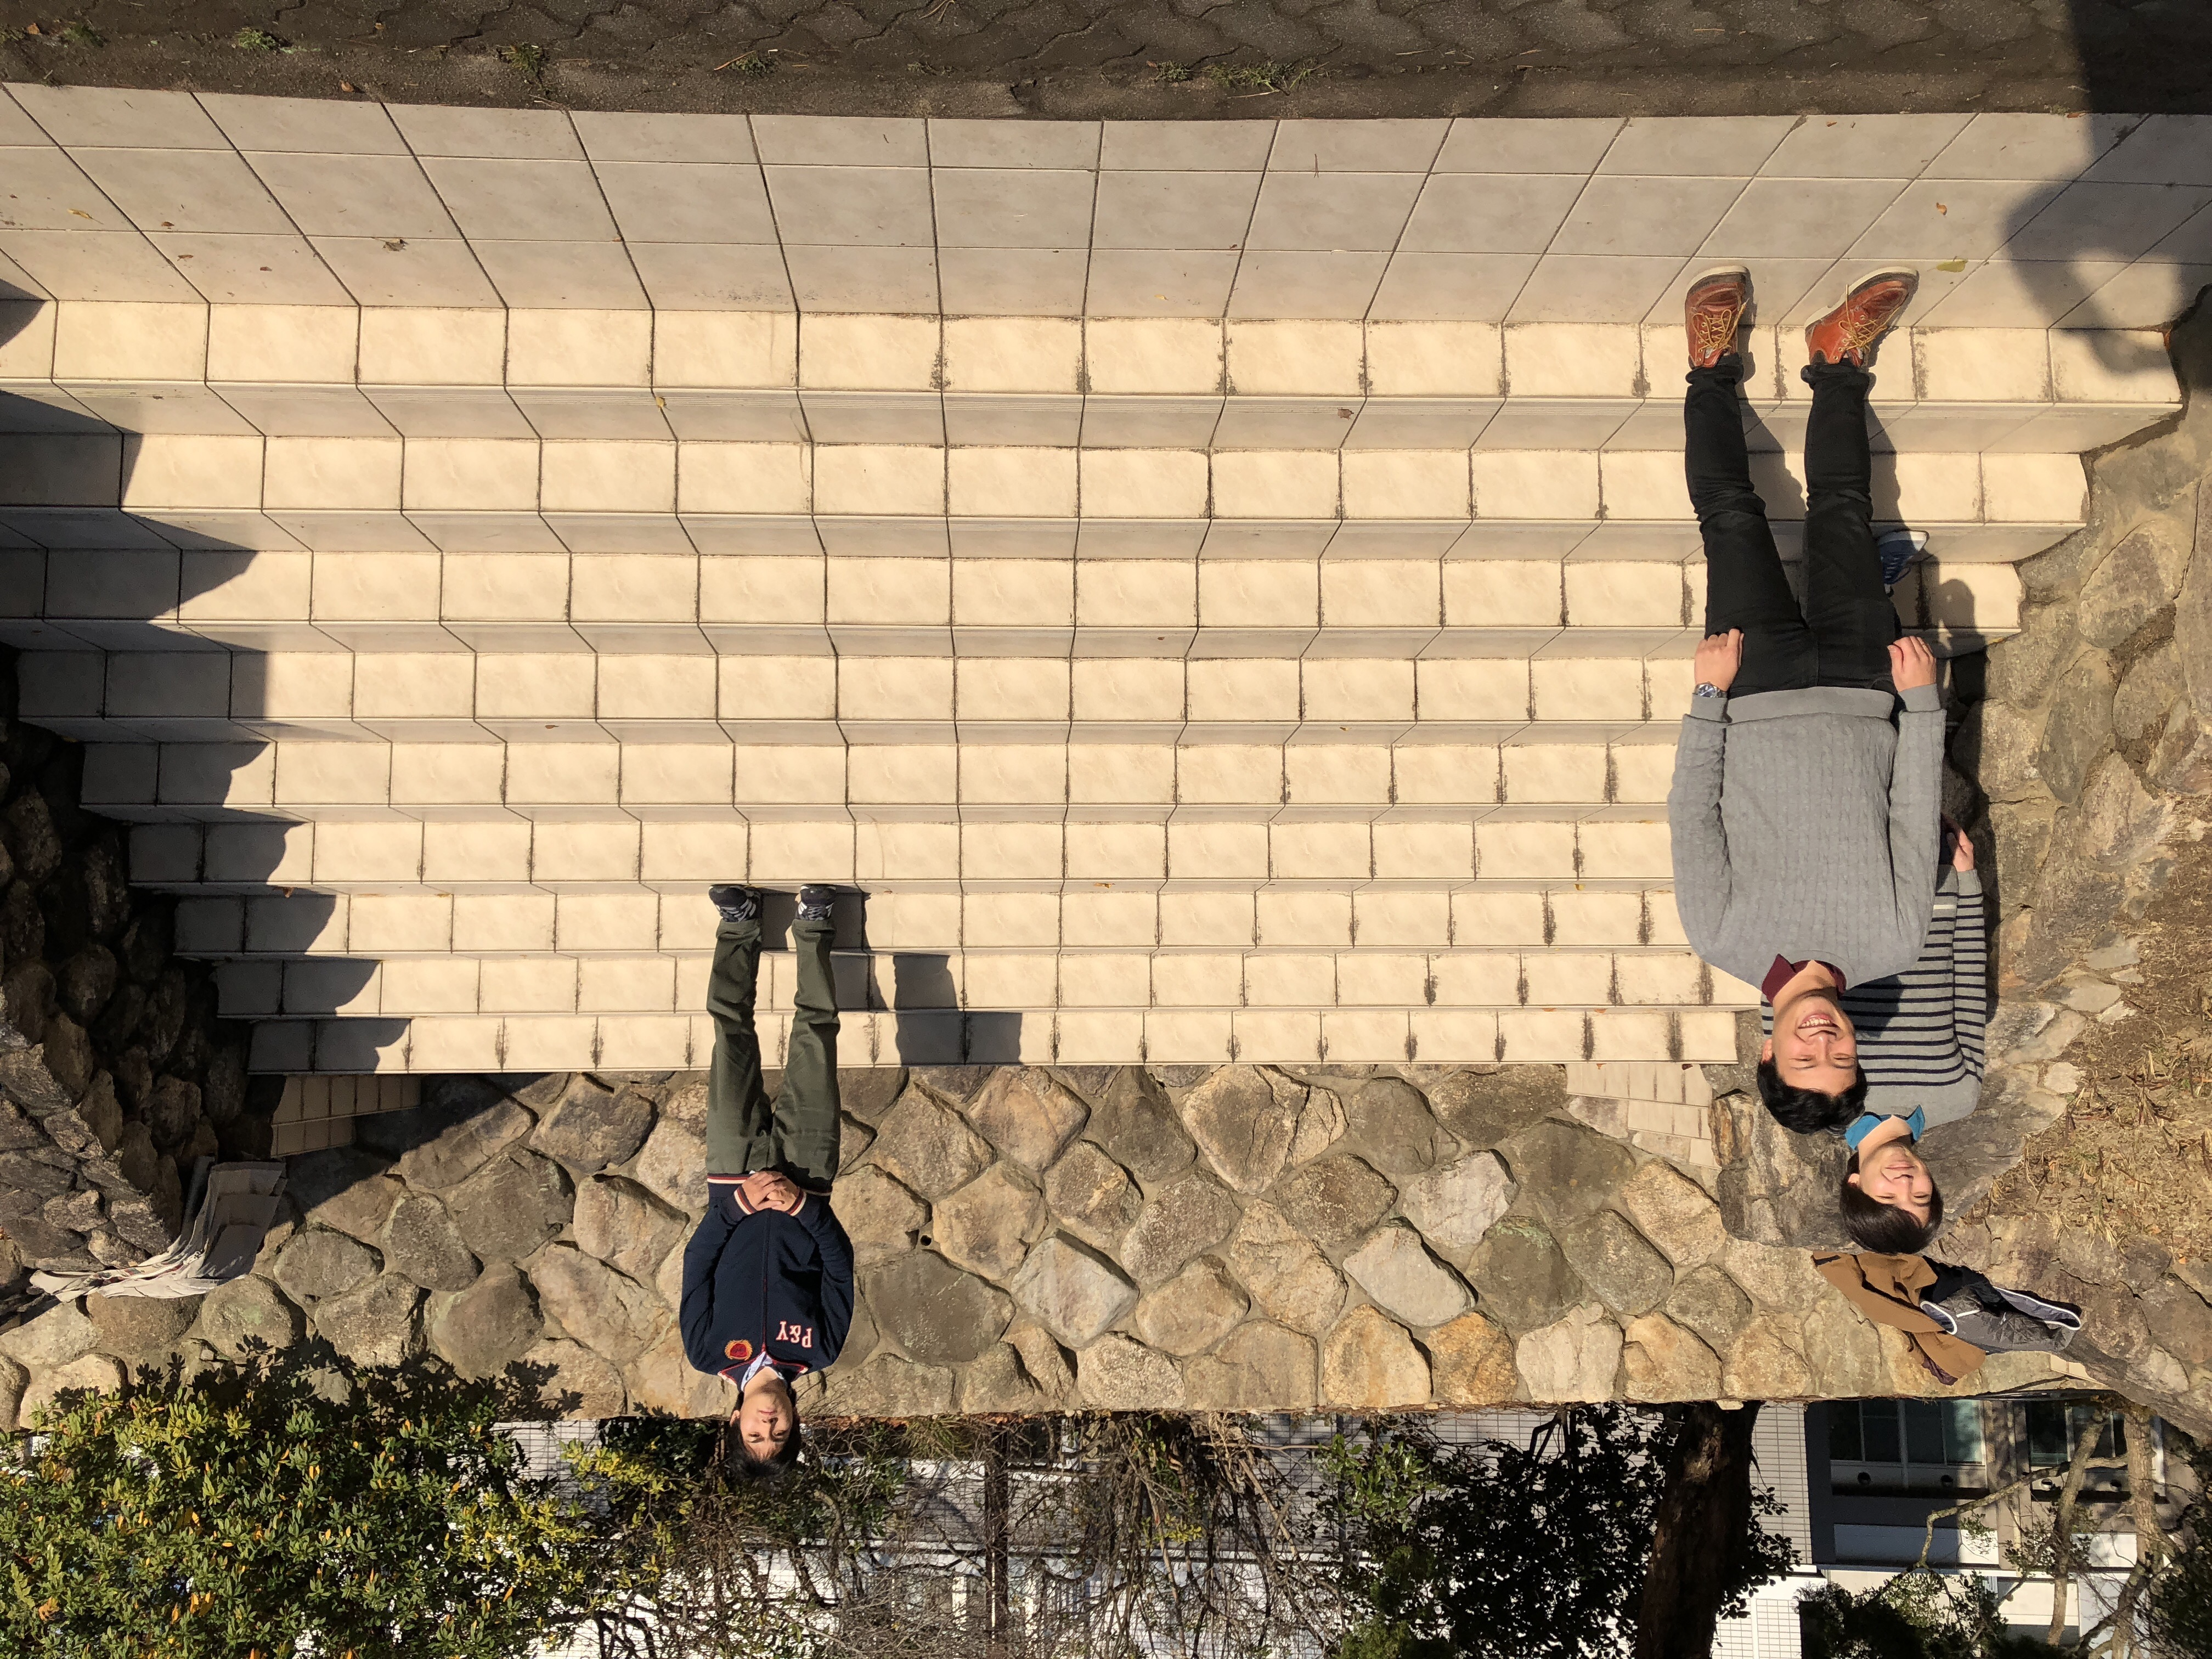
\includegraphics[scale=0.1]{na7}
\caption{第7次内閣}
\label{na7}
\end{figure}


%~~~~~~~~~~~~~~~~~~~~~~~~~~~~~~~~~~~~~~~~~~~~~~~~~~
\newpage
\section{Higengo International Symposium}
\subsection{第一回HIS}
\subsubsection{閉会の言葉}
はい、えっと、では閉会になりまして、今回第一回非言語国際シンポジウム、初の開催で大変好評で、有意義な議論になったと思います。
概念論文という人類の悲願を達成するために、私達は動いておりますが、そのために幾つもの犠牲を払っていくこととと思います。
特にATMや佐々木など、若干の被害は被る方はいらっしゃるでしょう。
我々はそれに屈してはいけません。
必ずや、概念論文を完成させ、次の時代の概念を切り開くためにがんばりましょう。
現在世界では、同時株安やテロの横行など、長く険しい道が待っています。
環境問題、宇宙開発の停滞、これらの問題に対し、非言語大学の概念が、新たな一歩を踏み出す、きっかけとなることを願っています。
最近では、日本でも政権交代が行われておらず、非常に概念が停滞し、うーん、しかし、えーっと、概念論文の存在がこの日本の停滞という概念が明るいものに変わることを祈っています。
最新の統計では、ノーベル賞受賞者の約8割が、我々の非言語大学の、概念に賛同を示しているというデータがありますが、我々がノーベル賞をとることも遠くないでしょう。
そもそもノーベル賞という概念は、あくまで、ノーベル博士がどうにかして作った賞に過ぎず、非言語賞という賞を、あの、非言語概念賞、こういったものを作って、より概念を高めた方に授与したいです。
例えば、非言語平和賞、非言語微分積分賞、また、非言語長編小説賞、非言語ラグビー賞、非言語エグザイル賞、オガワ教授が受賞予定でございます。
これらの賞を、取ったオガワ教授は、これからも概念論文のために尽くされ、最終的には、彼自身が新たな概念となることを祈っています。
要するに、世界平和を目指しましょう。
以上、私の閉会の挨拶と変えさせて頂きます。
\par
平成30年10月14日 非言語大学清掃員 又吉康平

%\begin{figure}
%\includegraphics[clip,scale=0.25]{Poster_1stHIS}
%\end{figure}

\begin{figure}[H]
\centering
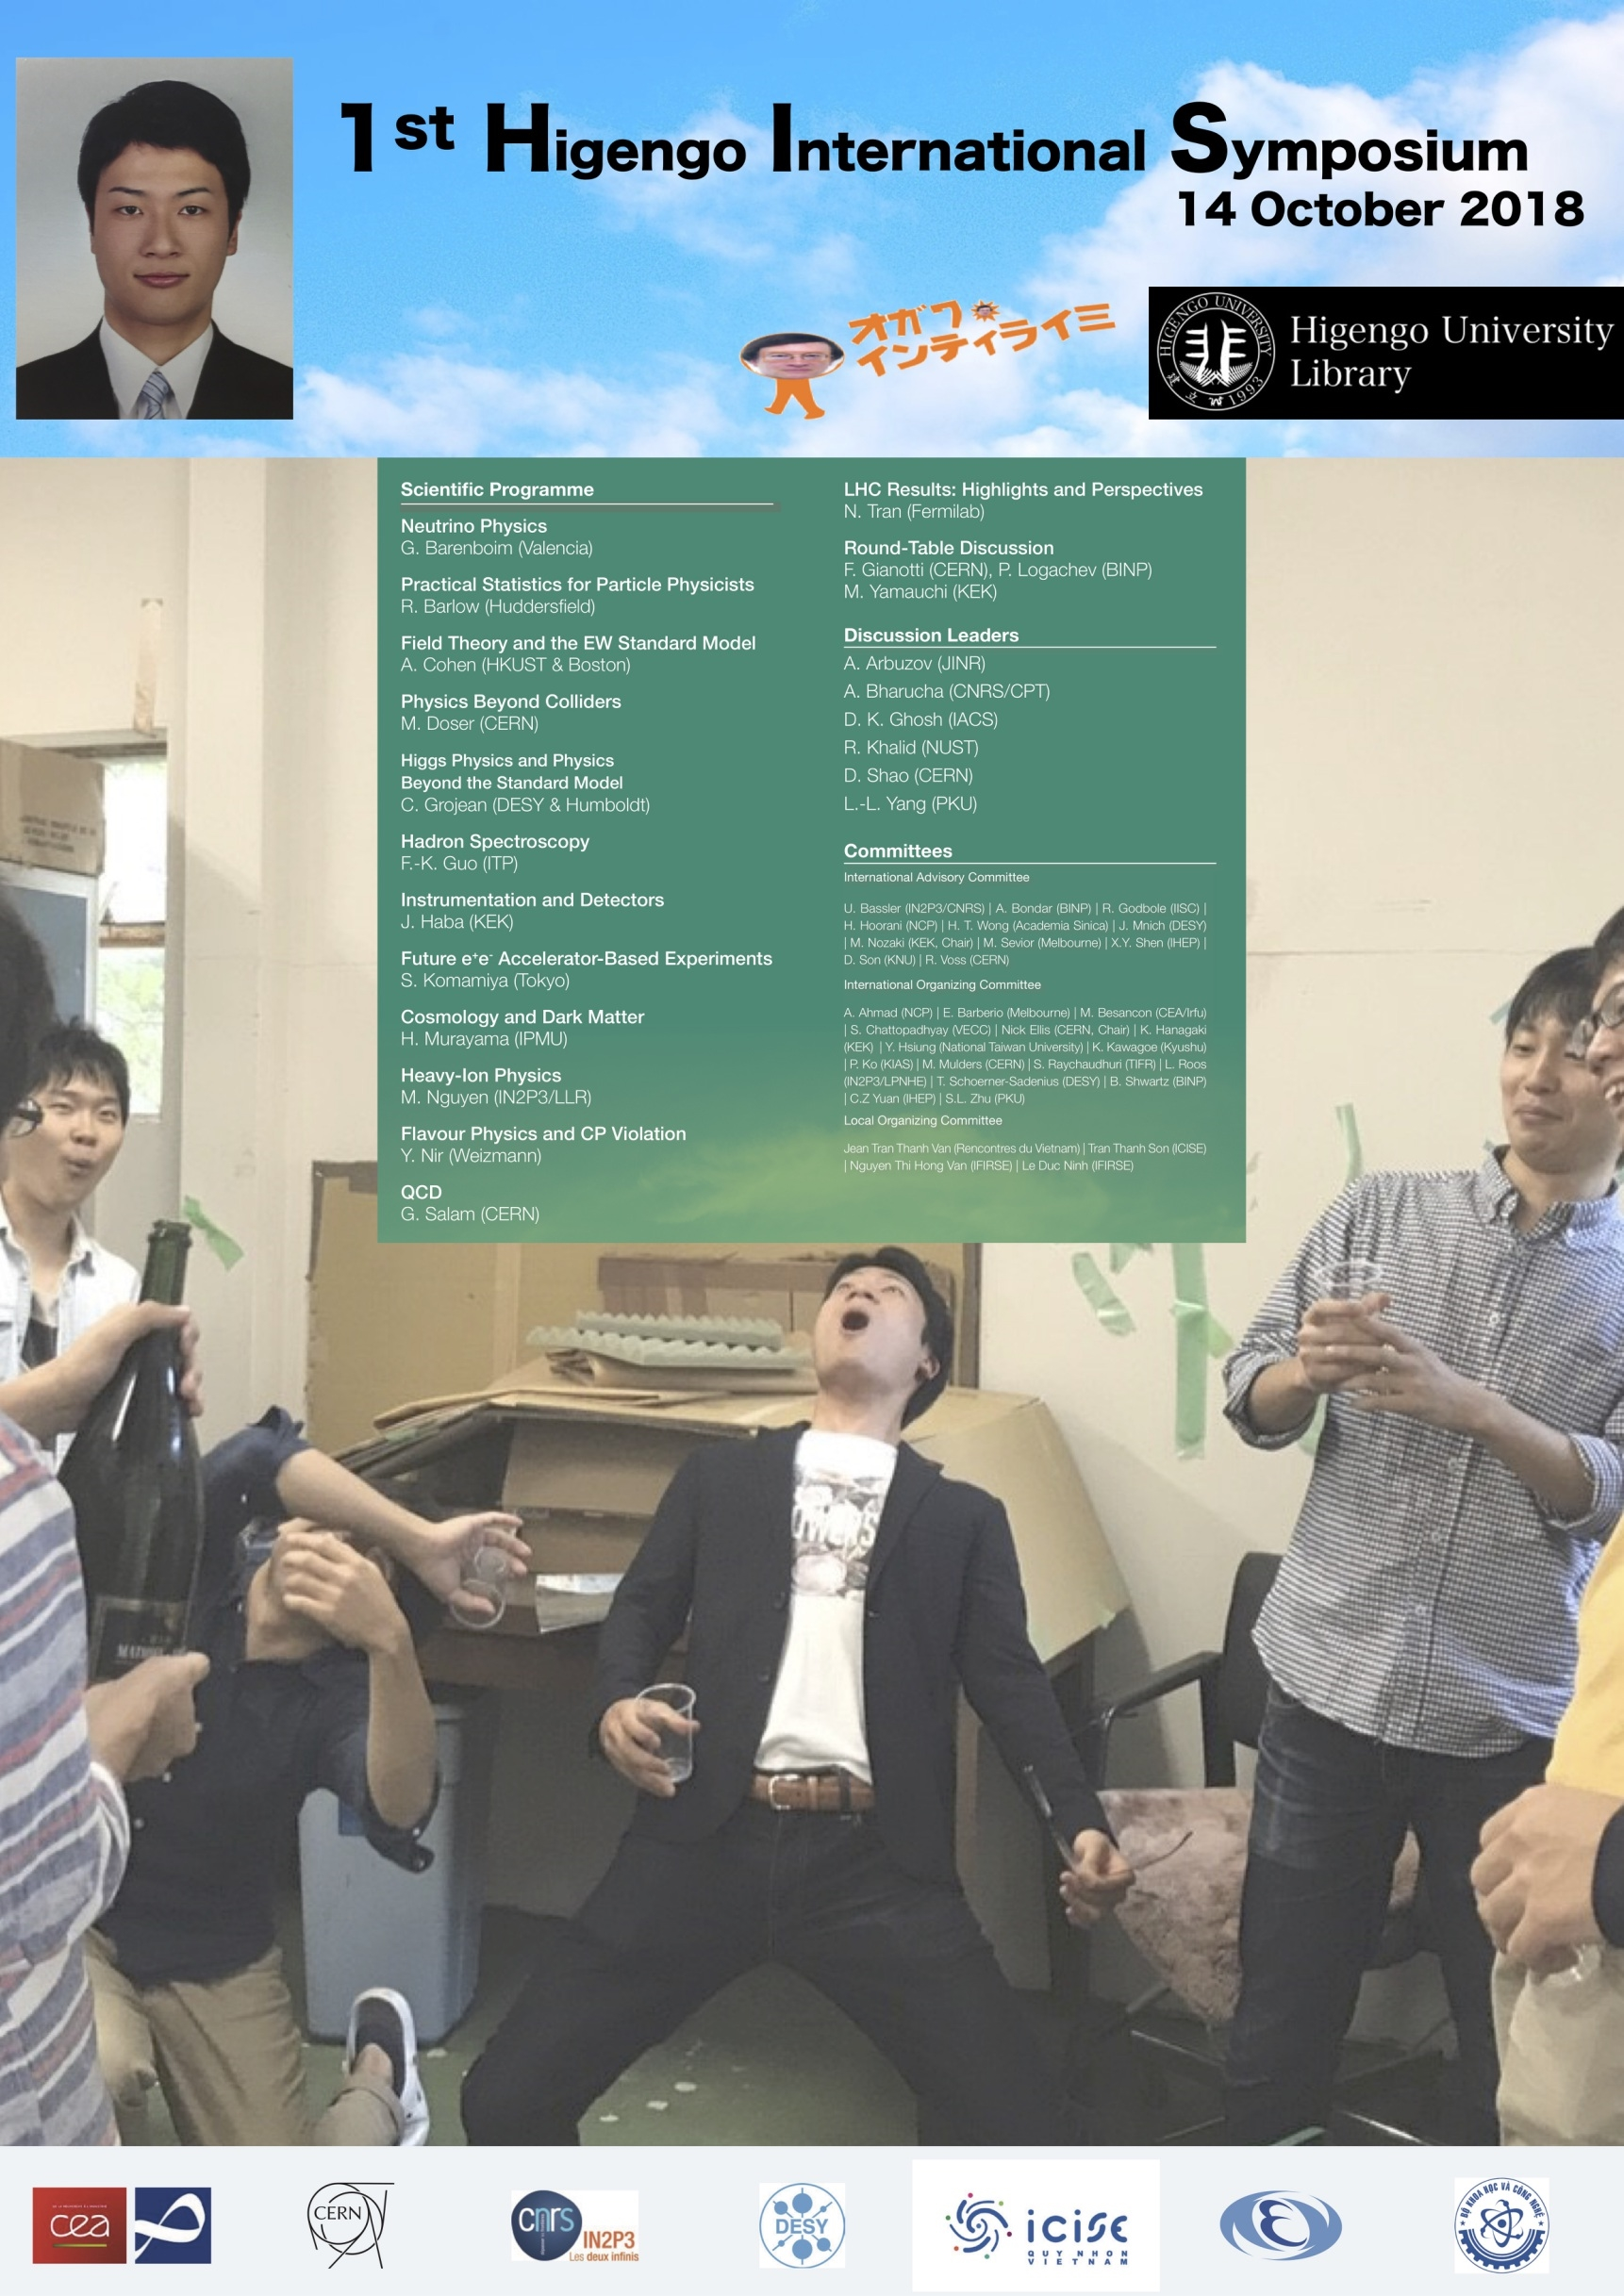
\includegraphics[scale=0.1]{HIS1.jpg}
\caption{第1回HISのポスター}
\label{HIS1}
\end{figure}

\subsection{第二回HIS}
\subsubsection{閉会の言葉}
えー、第二回HIS、開会おめでとうございます。
えー、今日はとてもよく晴れた秋晴れの日で、朝は寒く、皆様もお風邪などを召されぬよう、一部の人は風邪を引いたようですが、できる限りビタミンを取って、ビタミンD。
ビタミンといえば、レモン。レモンといえば、生牡蠣。生牡蠣といえば、カキフライ。カキフライといえば、タルタルソース。
みなさんもタルタルソースの様に、黄色く、色々な色が混ざった、ビタミンが入っているので黄色。
で、はい、原液のタルタルソースを飲むことで、風邪を引かない元気な体になります。
最近の研究で、タルタルソースを1日100mL飲むことで、寿命が15年も伸びる結果がでています。
韓国?
寒さがありますので、風邪などを引かぬよう。
風邪を引いてはいないんですけど、北海道ではないんですけど(琉球乃笑)。

前回は3人中2人が集まり、今回は1人も集まることができておらず、これも皆様の技術力が足りなかったから集まれなかったという、悲しい。
そうですね、誰が悪いかといえば、政府が悪い。特に、官房長官。
んー、あのひとはタルタルソースを取っていないから、良くない。
はい、そのせいで、日本とスイスが遠い。

学長がタルタルソースを取っているかどうかは私にはわかりませんが、最新の研究では歴代の学長の3割はタルタルソースを取っていなかった。
彼らはみな途中で、失脚して、ビタミンを取らないから失脚した。

前回のHIS、様々な新しい課題が発見され、例えば、宇宙の広さとか、宇宙の寒さとか、宇宙の重さとか、新しい課題が多くあり、はい、例えば、地球の広さとか、地球の重さとか、地球の人口は年々増えていますから。
んーー、はい、人類がこれからもよりよい文明をきづいていけるように、我々も頑張らなければなりません。

—特に印象的だったのは?
特に例えば、佐々木がビタミンを取っていないとか、アツムさんは取ってるけど、だからあの人は長生きします。
Road to 学長。
ぜひ、ビタミンを取って学長になっていただきたいです。
そう、願うばかりです。

そのような前回を経て、今回はより規模の大きい、ネットでLIVE中継されておりますから、まずは動員数1億、youtubeでも発信します。再生回数100億。今回はそのような気合を入れて、がんばりましょう。

\begin{figure}[H]
\centering
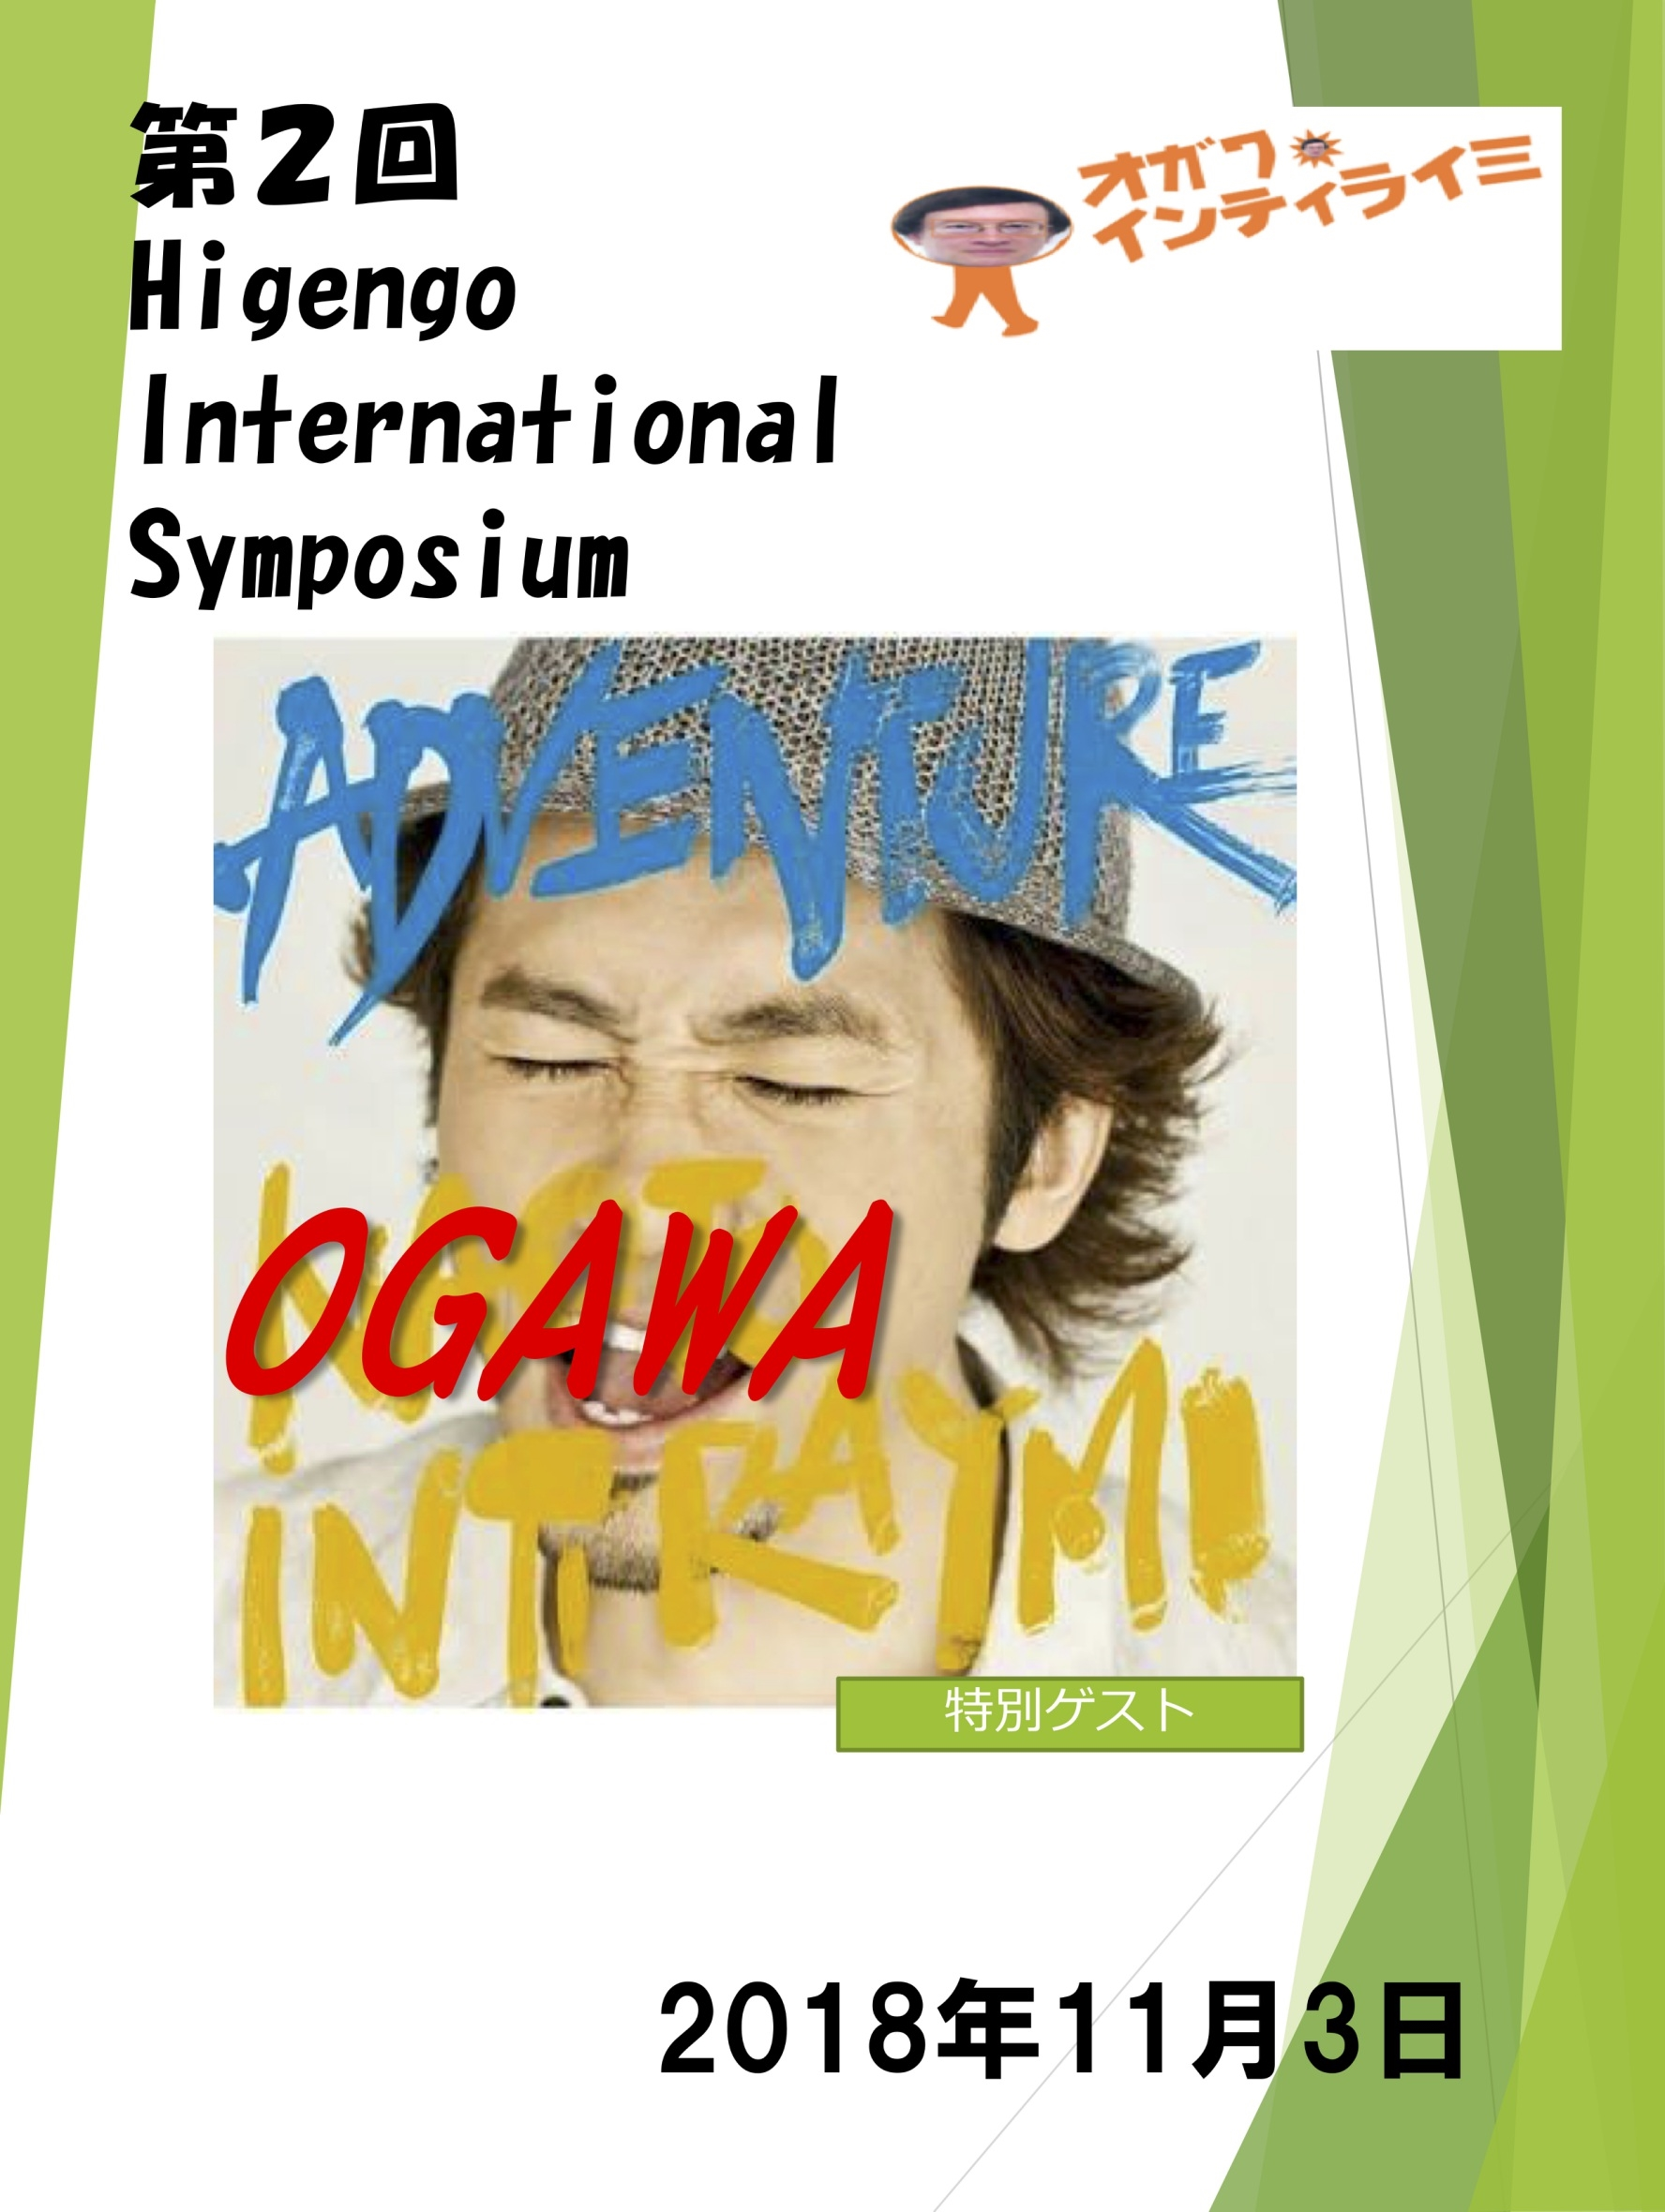
\includegraphics[scale=0.1]{HIS2.jpg}
\caption{第2回HISのポスター}
\label{HIS2}
\end{figure}


\subsection{第三回HIS}
\subsubsection{開会の言葉}
はい、よろしいでしょうか。おはようございます(CERN12時)。本日は、お日柄も、現在私のいるところは雨が降っているのですが、偶然にも皆さん雨が降っているようで、大変喜ばしいことではありますが、雨というのは古来より、豊作をもたらすとても演技の良い天気です。例えば、昔の人は、稲作をするのにも雨水を使いました。今は、そう、人工的な水を使っており、大変風情がなくなっております。えー、「晴耕雨読」という言葉が、晴れの日は畑を耕し、雨の日は本を読め。この続きとしまして、雪が降ったら雪合戦「雪投(せつなげ)」桜が散ったら一年生「桜一年」(おういちねん)、みなさんも桜が散るころには一年生。桜が散るまでは予備生。みなさんも桜の散るころを楽しみにしながら、雪の日は雪を投げ、ましょう。
日本最大の戦い、M-1グランプリ。特に、今回、活躍された、上沼恵美子さん、大変な話題をかっさらっていきました。特に、会場で、他の参加者を突き飛ばして舞台にたつという勇気、
- 北海道では放送されていたと?「はい」。「いいえ」。
今回優勝された、ジャルジャルが優勝してませんけど、えー、まぁ、残念ながらジャルジャルのネタは見ていないのですが、まぁジャルジャルという、えー、ジャルというのは飛行機の名前で、これはかれらの大空の飛び立つという強い気持ちがあり、とても勇敢な名前です。大変感動的なネタをしていらっしゃいました。見ていなくとも、感動できる、神の領域。また、優勝されたユニバース、は優勝されていませんが、えー、ユニバースというのは宇宙という意味ですね、えー、まさに宇宙のような広大な世界観をもったネタを披露していただきました。たしか、見ました。点数でいうと、残念ながら、70点と。なぜ彼らがこの舞台に立てたのか、裏口入学。これは大変な、不正であり、私は、この件について裁判所に提訴しました。その結果、ユニバースのお二人は残念ながら、えー、体調をくずされました。来年、出場はできないと、なってしまいました。これはさすがに、やりすぎたかなと反省しております。見事、優勝された、かまいたち、ではないけども、えー、かまいたちというのは、イタチですね。イタチがコンビを組み、イタチでした。大変めずらしいお笑いコンビ。まぁ、日本語は喋れていました。当然イタチなので、マイクに届かず、若干聞き取りづらい場面が残念でした。これを受けまして、M-1グランプリは人間以外の参加者に優しくないという、弱点が浮き彫りになりました。今後は、イタチのような参加者にも配慮した、バリアフリー設計が求められております。
はい、そして、流行語大賞。今年の流行語大賞は、
第5位「日産雨読(太陽の出ているときは生産に励み、雨の降っているときは本を読む。屋根がない、しょうがない)」
第4位「プリクラ(これは、中高生の間で大流行、プリ:プリン体、クラ:藏重、ビールなどの飲み過ぎで若干不健康。例えば、街でプリクラを見かけると写真を撮る。プリクラは、まぁ諸悪の根源はアルコール。ドラマの影響、「霜降り和牛」の影響。)」
第3位「米津(米津玄師と似ているナオト・インティ・ライミに由来する。名曲:富士山。主に男子小学生に人気。全国の小学校で配布したという、その御蔭でブームに火が付いた。ちなみに、ナオト・インティライミの最新曲は、スタートトゥレイン。これは、ナオト・インティライミも晴耕雨読を実践しているということですね。)」
第2位「おかき体育(有名なオカキ体育。これは、まさに言わずもがな。)」
第1位「晴耕雨読(晴れた日には畑を耕し、雨の日は、人の心を読む。大変ミステリアスな言葉。これは映画で流行りました。全世界で上映されました。「君の名は。」という映画ですが、岡崎体育が主演を努めました。ヒロインは、ミラ・ジョボビッチ。制作はインドで行われました。踊るという愉快な映画。その中で、晴耕雨読という言葉が多用されておりました。主人公の口癖は、おれは明日、晴耕雨読。おれは晴れても雨が降っても対応できる、素晴らしい言葉です。晴れた日には本読み、違う。雨の日には畑を耕す。雪が降れば雪を溶かし、桜が散れば、卒業シーズン。海が開けば、古代エジプトのモーセの十戒。めでたいイベントが起こります。まず、総興行収入2000万元/国×96ヶ国、数え方によっては200ヶ国。人々の心を癒やした。紛争地域の人々も明日から畑を耕そう。5000兆ドル。まぁ少し前までは、中国が強かった。この計算したときはアメリカが強かった。一説には裏口入学。提訴に関して、秘密裏に動くこととしました。その結果、現在私は国連に監禁されております。国連本部地下30階に幽閉されております。今後はまず、脱獄。ステップ1:看守を倒して鍵を奪う。ステップ2:エレベーターで地上まで。)」
というわけで、今回のHIS、意気込み、大変盛り上がっております。これまでに培われた情熱と技術を存分にぶつけあって、歴史に残る会議にすることができれば良いと考えています。
では、ここに第3回HISの開会を宣言します。

\subsubsection{閉会の言葉}
えー、お疲れ様でした。この四字熟語を送ります。
\[
朝三暮四
\]
これは、朝が3つ、夕方3つ、夜は200個。これは朝は軽く、夕方も軽く、夜は一杯だべる。すなわち、夜型生活。みなさんも健康に気をつけて、暮らしましょう。
では、今回の第三回HISを閉会します。

\begin{figure}[H]
\centering
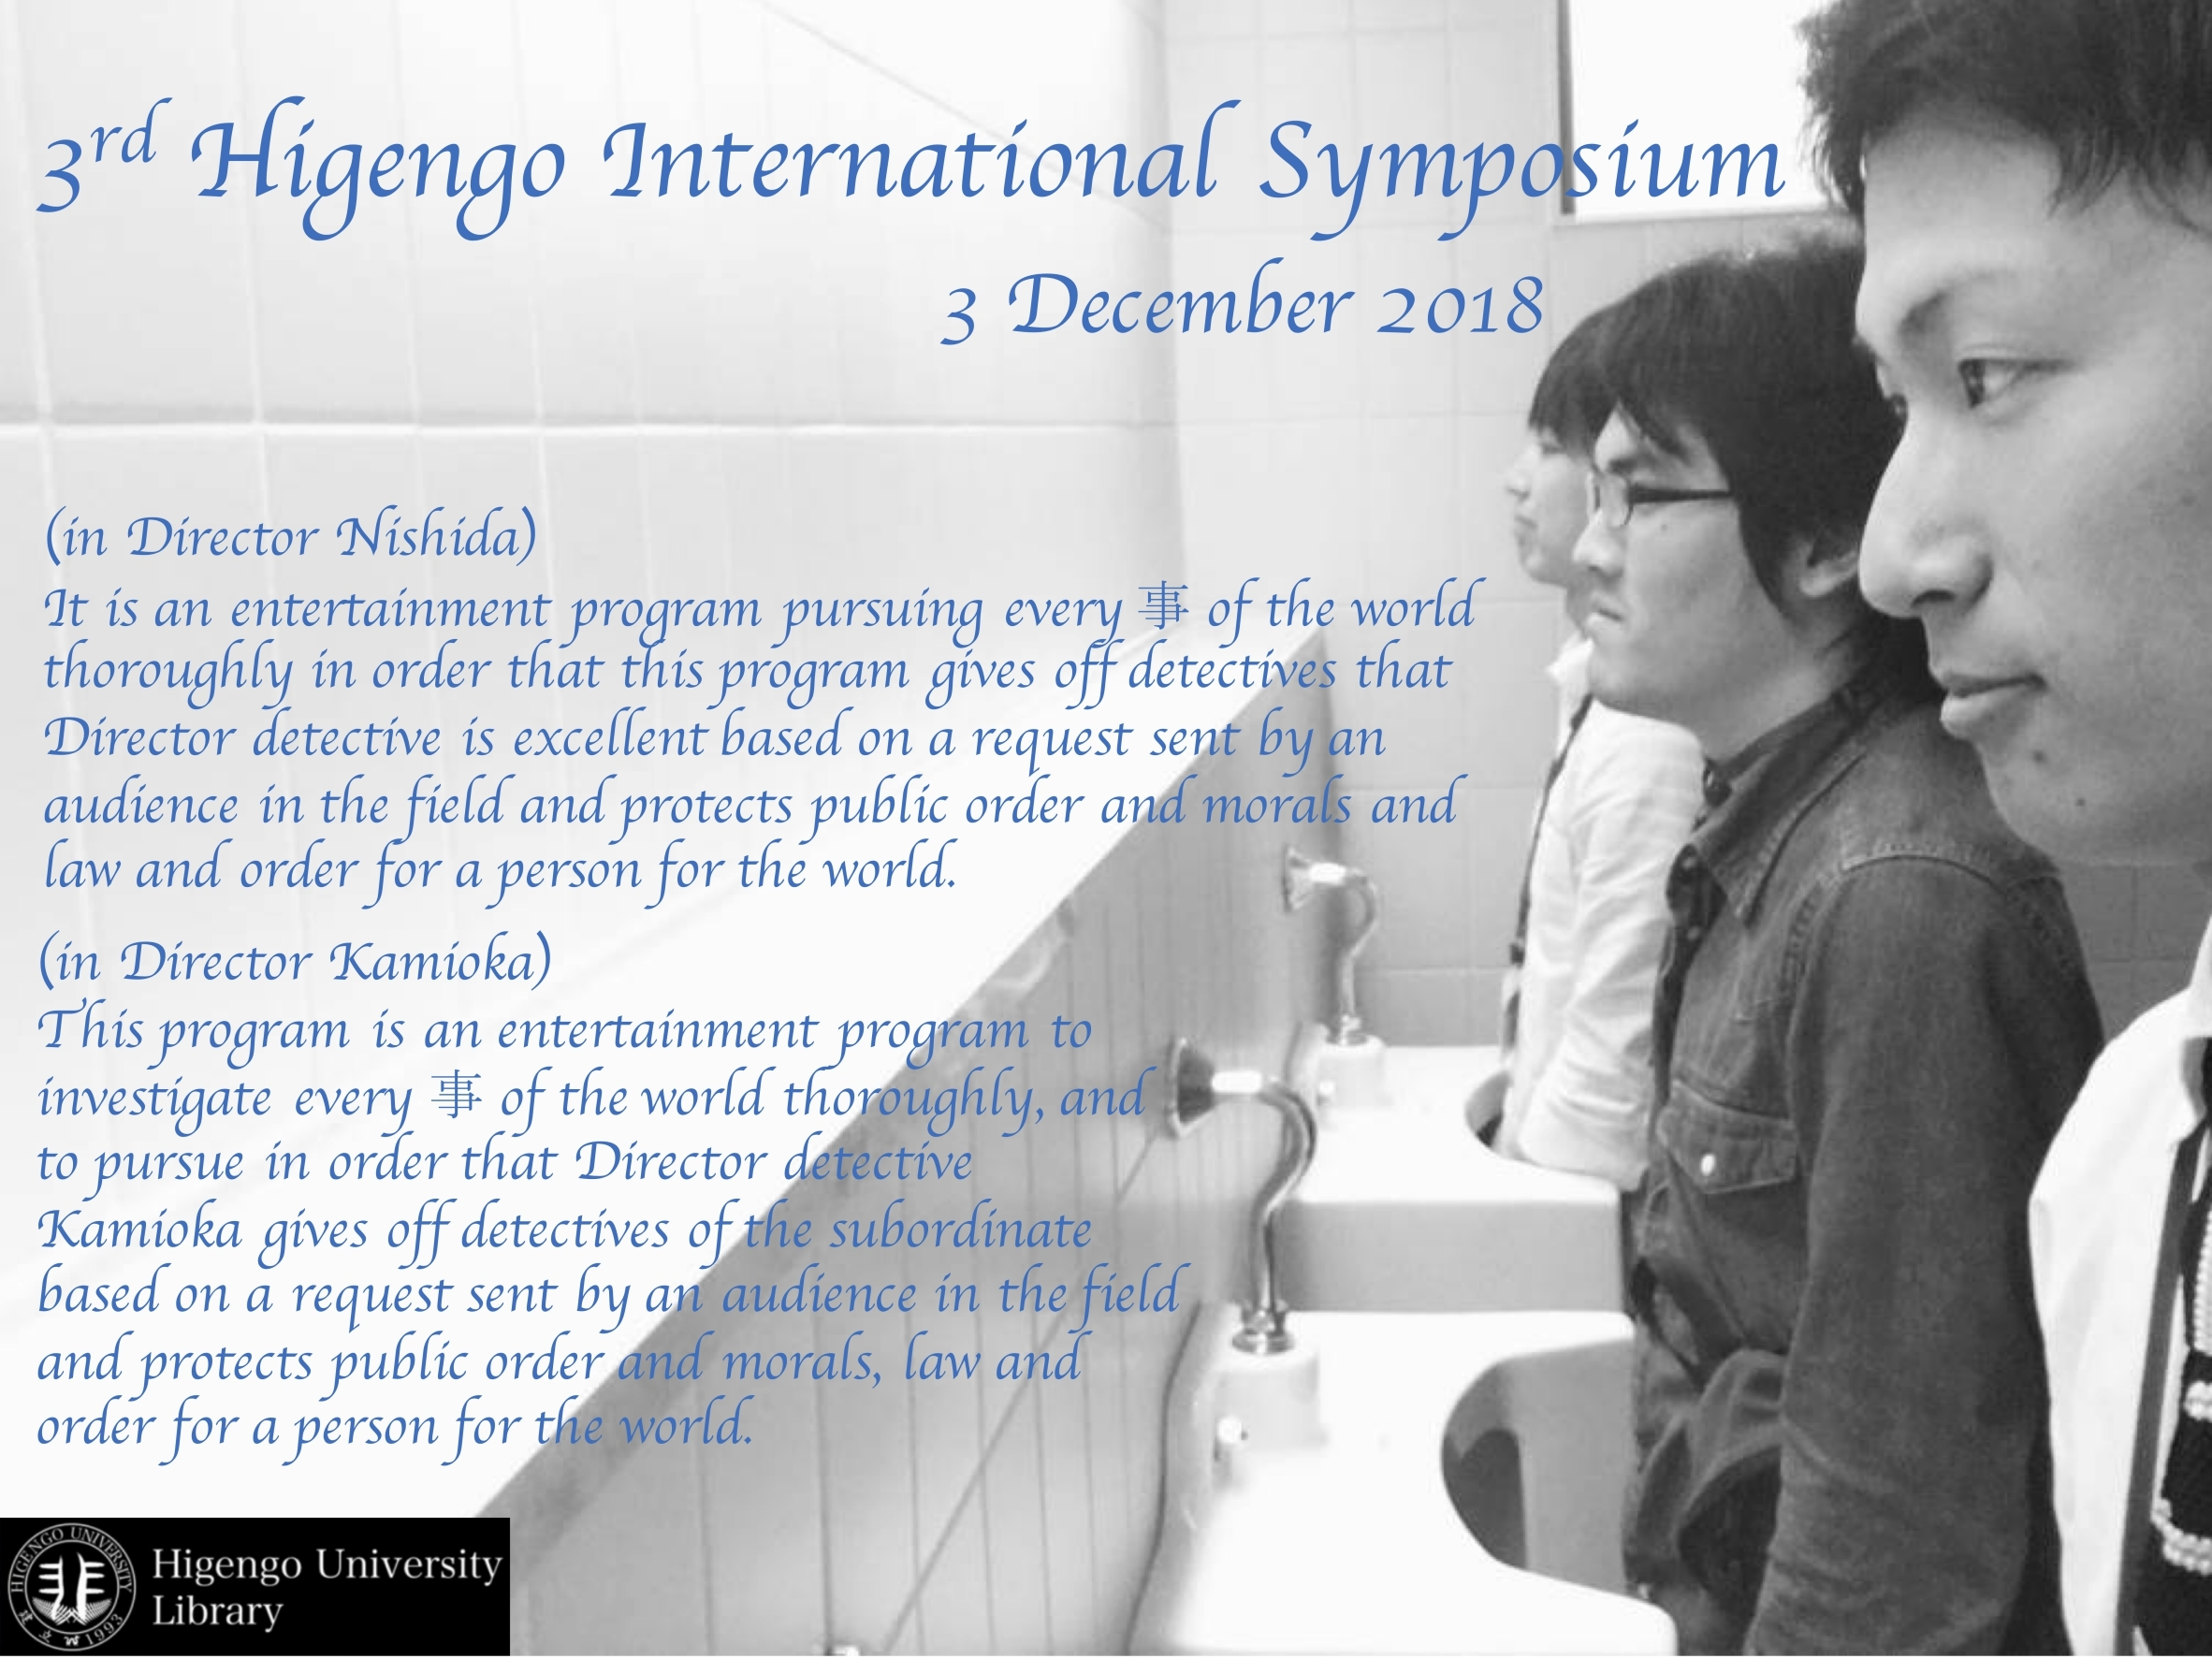
\includegraphics[scale=0.1]{HIS3.jpg}
\caption{第3回HISのポスター}
\label{HIS3}
\end{figure}

\subsection{第四回HIS}
都合により、又吉清掃員は欠席した。

\begin{figure}[H]
\centering
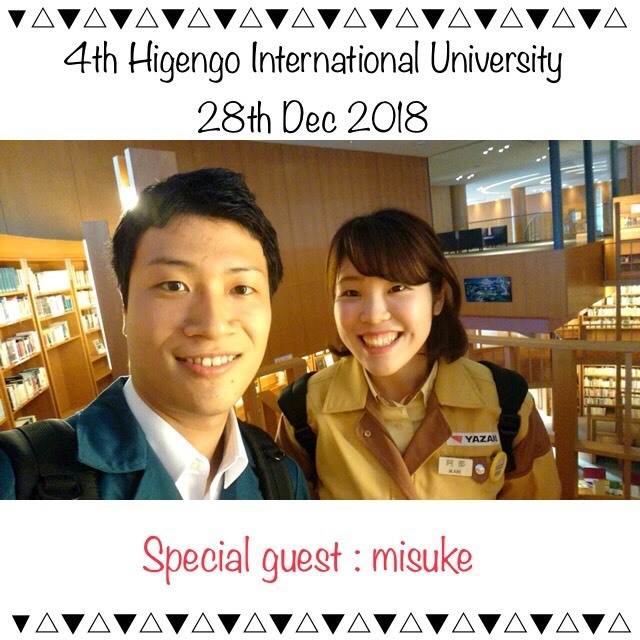
\includegraphics[scale=0.5]{HIS4.jpg}
\caption{第4回HISのポスター}
\label{HIS3}
\end{figure}


\subsection{第五回HIS}
\subsubsection{開会宣言}
はい、えー、第五回HISということで初めて三人が顔を合わせての物理的なHISとなりました。
まぁ第四回は三回sてないのでわからないですが、(謝罪要求)、第四回については、私が南極に出張中、ペンギンの清掃をしておりました。
そこであったこととは?
南極でペンギンの体を拭いていたとき、現地の方がカップレーマンエオ分けてくださいました。
そのカップラーメンというのが、日進のあれ、当時しばらく日本食を食べていなかったので、日本を感じられるあたたかさ、
半分ペンギンに分けたのですが、生石層に食べていました。
代わりに魚を半分もらいました。アジフライにして食べました。
アジフライといえば?そう、南極にも当然あじはいらっしゃいます。
南極の氷を掘ると、氷の中にアジがいる。
現地の方が、アジを埋めている。現地の方からペンギンに譲られて、私がもらいました。
現地の方はペンギンをとても大事にしている。
全南極のペンギンの半分のアジをもらいました。
半分だけ食べました。つまり、大体3匹ほど。南極のペンギンは5〜6匹ほど。
いや、まぁ、ペンギンはとてもつつましく暮らしており、シャイである。
もういったことがありまして、第四課には参加できなかった。

第一回に引き続き、神戸で開催されると。
ポートタワーが有名ですが、はい。
ポートタワーは赤い、赤いといえば狐、きつねと言えば、今年のセンター試験には狐が出てきたそうで。
センター試験を受けているということで、このような場で開会宣言をできることを嬉しく思っております。
いまセンター試験を受けている学生のみなさん、日頃の努力を信じて、どんな結果であっても、目指せ東進。
東大に進学する。
赤いもんが有名、赤いもんといえば浅草、浅草いったことないんですけど、
せんべいとか、ありますけど。食べてはいないんですけど。
浅草といえば、こち亀。
こち亀最後は、世界大戦が勃発して、両さんが戦争に行くということで、悲しいお話。
ファンとしては、最後は、やはり明るく終わっていただきたかった。
まぁ、当時連載をした当時は、戦争で悲しいお話が多かったですが、そういったお話になってしまったそうです。悲しい。

えー、で、第五回の意気込み。ということで、ついにこのときが来たかと。
いよいよ、あらまぁ、いろいろと終わりを迎える時期でもあります。
完成というか、卒業、HISを卒業。その先に、進学。
HISを卒業されるみなさんも、これからセンター試験がまっていると思いますが、センター試験は頑張ってください。
そのあと、それぞれ思い思いの大学に行くなり、就職するなり、センター試験をまた受けるなり。
気が向けばHISにまた戻ってきていただくこともできます。
HISではみなさんの健全な心の育成を目指してきました。
ここで学んだ強い気持ちを、皆さん忘れずに。
えー、より高みへ。
高みー(ジ・アルフィー)を目指して、新世代のジ・アルフィーを。
ジ・アルフィーツー。スリーフォーとどんどん続いていけばいいなと。
私は、ジ・アルフィーゼロなんですけど。
メンバーは、タカミー、私のジ・アルフィーゼロ。
あとドラムの、えー、佐々木ユタカ。
あと、ボーカルの、小栗瞬。
私は清掃員です。
それから、タカミーはピアノです。
ギターが、フレディ・マーキュリーさんという名前のフィリピン人です。偶然にも名前が同じ。
ベースは、ジョブズ。ジョブズさんは最近ちょっと、まぁ、脱退されて。
タカミーはずっと頑張ってます。
その他の方々は諦めている。
もともとドーム公演を目指していたのですが、やがてメンバー間に確執が。
特に小栗瞬が俳優デビューしたいと、私は無理だと止めたのですが、小栗瞬はやるんだといってハリウッドへ。
日本にも似たような名前の俳優さんがいらっしゃいます。
彼は頑張っていらっしゃいます。

まぁ、ジ・アルフィーゼロのメンバーは皆さん、HISの関係者。
HISにはたくさんの裏方がいらっしゃいますが、彼らは舞台裏にいます。
こういった皆さんに支えられて、参加できていると。

第五回の意気込み。
こういって支えられたHISもついに第五回。つまり、DAIGO。まぁダイゴ。
千鳥は関係ありません、
第五回。
ダイゴと言えば、えー、まぁ政治にも力がある。
HISもついに政治進出。
次の参議院選挙に、誰か出馬させる予定です。
私は出ません。私はあくまで清掃員です。
政治の表舞台に立つなら、タカミー。
というわけで、タカミーの選挙必勝を祈って、皆さんで応援してください。

以上、第五回HISの開会宣言とします。

\subsubsection{ポスター}
第五回用のポスターは都合により割愛させて頂く。


